\documentclass[11pt]{article}

\usepackage[margin=1in]{geometry}
\usepackage[T1]{fontenc}
\usepackage[utf8]{inputenc}
\usepackage{lmodern}
\usepackage{microtype}
\usepackage{amsmath,amssymb,amsthm,mathtools}
\usepackage[makeroom]{cancel}
\usepackage{graphicx}
\usepackage{float}
\usepackage{placeins}
\usepackage{booktabs}
\usepackage[hypcap=false]{caption}
\usepackage{subcaption}
\usepackage{tikz}
\usepackage{pgfplots}
\pgfplotsset{compat=1.18}
\usepackage{enumitem}
\usepackage{xcolor}
\usepackage{csquotes}
\usepackage{array}
\usepackage{multirow}
\usepackage{changepage}
\usepackage{hyperref}
\usepackage[nameinlink,noabbrev]{cleveref}

\crefformat{equation}{(#2#1#3)}
\Crefformat{equation}{(#2#1#3)}
\crefrangeformat{equation}{(#3#1#4)--(#5#2#6)}
\crefmultiformat{equation}{(#2#1#3)}{ and (#2#1#3)}{, (#2#1#3)}{ and (#2#1#3)}

\pgfplotsset{
    myplotstyle/.style={
        width=4.9cm, height=4.9cm,
        axis lines=left,
        xlabel={$S$},
        xmin=0, xmax=1, ymin=0, ymax=1,
        xtick={0,0.5,1}, ytick={0,0.5,1},
        grid=major, grid style={dashed, gray!30},
        samples=100, domain=0:1,
        thick,
        tick label style={font=\tiny},
        label style={font=\small}
    }
}

\setcounter{topnumber}{4}
\setcounter{totalnumber}{6}
\renewcommand{\topfraction}{0.9}
\renewcommand{\textfraction}{0.1}
\renewcommand{\floatpagefraction}{0.8}
\makeatletter
\setlength{\@fptop}{0pt}
\setlength{\@fpsep}{8pt plus 2fil}
\setlength{\@fpbot}{0pt plus 1fil}
\makeatother

\setcounter{secnumdepth}{3}
\setcounter{tocdepth}{2}
\allowdisplaybreaks
\setlength{\parindent}{1.2em}
\setlength{\parskip}{0.15em}

% Thesis-compatible macros (AA)
\newcommand{\pgf}{probability generating function}
\newcommand{\intinf}{\displaystyle\int_0^{\infty}}
\newcommand{\pr}[1]{{\text{Pr}\left\{#1\right\}}}
\newcommand{\mean}[1]{{\rm I}\!{\rm E}(#1)}
\newcommand{\rr}{{\bf R}}
\newcommand{\xx}{{\bf X}}
\newcommand{\xt}{{\xx_t}}
\newcommand{\yy}{{\bf Y}}
\newcommand{\yt}{{\yy_t}}
\newcommand{\ww}{{\bf W}}
\newcommand{\wt}{{\ww_t}}
\newcommand{\xs}{{\xx_s}}
\newcommand{\vv}{{\bf V}}
\newcommand{\vt}{{\vv_t}}
\newcommand{\dd}{{\rm d}}
\newcommand{\dt}{{\rm d}t}
\newcommand{\ee}{{\rm e}}
\newcommand{\ddt}[1]{\displaystyle\frac{\dd #1}{\dd t}}
\newcommand{\dda}[2]{\displaystyle\frac{\dd #1}{\dd #2}}
\newcommand{\pddt}[1]{\displaystyle\frac{\partial #1}{\partial t}}
\newcommand{\pdd}[2]{\displaystyle\frac{\partial #1}{\partial #2}}
\newcommand{\dds}[1]{\displaystyle\frac{\dd #1}{\dd s}}
\newcommand{\ex}[1]{\mathbb{E}\left(#1\right)}
\newcommand{\de}{differential equation}
\newcommand{\rv}{random variable}
\newcommand{\delt}{\Delta t}
\newcommand{\ft}{\textit{F.~tularensis}}
\newcommand{\yp}{\textit{Y.~pestis}}
\newcommand{\Vt}{_{\text{total}} V}
\newcommand{\Ic}{ I_{\text{const}}}
\newcommand{\lb}{\left(}
\newcommand{\rb}{\right)}
\newcommand{\lrb}[1]{\lb#1\rb}
\newcommand{\lbs}{\left[}
\newcommand{\rbs}{\right]}
\newcommand{\lrbs}[1]{\lbs#1\rbs}
\newcommand{\xdt}{{\xx_{t+\delt}}}
\newcommand{\zz}{{\bf Z}}
\newcommand{\ydt}{{\yy_{t+\delt}}}
\newcommand{\pt}{p_{i,j}(t)}
\newcommand{\p}{p_{i,j}}
\newcommand{\lbc}{\left\{ }
\newcommand{\rbc}{\right\} }
\newcommand{\lrbc}[1]{\lbc#1\rbc}
\newcommand{\lrbq}[1]{\hspace{-2pt}\lb#1\rb}
\newcommand{\Id}{{I_{\text{death}}}}
\newcommand{\pdx}[2]{\displaystyle\frac{\partial #1}{\partial #2}}
\newcommand{\pdxn}[3]{\displaystyle\frac{\partial^{#3} #1}{\partial {#2}^{#3}}}
\newcommand{\eec}{{\ee^{\lambda(a-b)t}}}
\newcommand{\Eqref}[1]{Eq.~\eqref{#1}}
\newcommand{\Figref}[1]{Figure~\ref{#1}}
\newcommand{\Tabref}[1]{Table~\ref{#1}}
\newcommand{\Chapref}[1]{Chapter~\ref{#1}}
\newcommand{\Secref}[1]{Section~\ref{#1}}

\theoremstyle{plain}
\newtheorem{theorem}{Theorem}[section]
\newtheorem{proposition}[theorem]{Proposition}
\newtheorem{lemma}[theorem]{Lemma}
\newtheorem{corollary}[theorem]{Corollary}
\theoremstyle{definition}
\newtheorem{definition}[theorem]{Definition}
\theoremstyle{remark}
\newtheorem{remark}[theorem]{Remark}

\hypersetup{
  colorlinks=true,
  linkcolor=blue!55!black,
  citecolor=red!55!black,
  urlcolor=blue!60!black,
  pdftitle={Mathematical introduction},
  pdfauthor={Adam Aldridge}
}

\title{Mathematical introduction\\[4pt]\large Branching, quasi-stationarity, and absorption}
\author{Adam Aldridge}
\date{Chapter~2\\University of Leeds}

\begin{document}

\maketitle
\vspace{-1.5em}

\tableofcontents
\clearpage

\section{Introduction}
\label{sec:intro}

The models in this thesis track populations that are small enough for chance to be part of the mechanism. A few colony-forming units deposited in a mammalian host, a handful of intracellular pathogens inside a single cell: in each case the count lies far from the regime in which deterministic rate equations describe what actually happens. The questions that matter --- will the population establish at all? if it survives, how large is it typically? --- are questions about distributions and rare surviving trajectories, not about a single mean path. This chapter assembles the mathematical apparatus needed for those questions.

Two threads organise the material that follows.

The first is \emph{conditioning on survival}. A subcritical branching process dies out almost surely, so its unconditional mean decays geometrically and carries little information about what a surviving realisation looks like. Restricting attention to those trajectories still alive at generation \(n\) produces a different picture: the conditional population settles to a fixed law, the \emph{quasi-stationary} (or Yaglom) distribution, whose mean is a constant. For the binary Galton--Watson process with replication probability \(p<\tfrac12\) that constant is \(1/A(p)\), where
\begin{equation*}
A(p) = \lim_{n\to\infty}\frac{S_n}{(2p)^n},
\end{equation*}
and \(S_n\) is the probability of survival to generation \(n\). A substantial part of the chapter is devoted to \(A(p)\): exact representations, bounds, near-critical asymptotics, comparison with the continuous-time analogue, and the dynamical reason why no elementary closed form is known.

The second thread is the \emph{near-critical regime}. As \(p\) approaches \(\tfrac12\) from below, extinction becomes slow, the quasi-stationary mean \(1/A(p)\) diverges, and any numerical scheme that relies on iterating to stationarity becomes expensive. Just above \(\tfrac12\), the size of the founding cohort weighs heavily on the chance of ultimate survival. Behaviour on either side of criticality is what makes small inocula scientifically interesting and computationally awkward.

\Cref{sec:prelim} records the continuous-time and generating-function language used later. \Cref{sec:gw} sets out the Galton--Watson process and the two facts on which the discrete analysis rests: extinction is certain at and below criticality, and at criticality the expected lifetime is nevertheless infinite. \Cref{sec:qsd} derives the limiting conditional mean and variance and introduces \(A(p)\). \Cref{sec:small} treats a founding cohort of size \(k\), records discrete birth--death--catastrophe survival formulae, and gives the continuous-time birth--death constant \(A_{\mathrm{c}}(p)\), for which a closed form is available. \Cref{sec:Ap} develops \(A(p)\) in full. \Cref{sec:moc} turns to absorption models and the method of characteristics for the generating-function partial differential equations used in later chapters when particles move between extracellular and intracellular compartments.

Standard results are presented as such. Heuristic steps and places where numerics carry the argument are marked. Where a claim can be checked numerically, it has been.

\section{Mathematical preliminaries}
\label{sec:prelim}

This section fixes notation and the continuous-time language used for absorption models and birth--death processes later in the chapter. It is not a survey of probability: only those objects that reappear in subsequent sections are stated.

\subsection{Exponential clocks and competition}
\label{sec:exp}

\begin{definition}[Exponential law]
A non-negative random variable \(T\) is exponential with rate \(\lambda>0\), written \(T\sim\mathrm{Exp}(\lambda)\), if
\begin{equation*}
\pr{T>t}=\ee^{-\lambda t},\qquad t\ge0.
\end{equation*}
Then \(\mean{T}=1/\lambda\) and \(\mathrm{Var}(T)=1/\lambda^2\).
\end{definition}

The exponential law is memoryless: \(\pr{T>t+s\mid T>s}=\pr{T>t}\). Consequently, in continuous-time jump models, the waiting time until the next event can be redrawn from the current state without reference to the past.

\begin{proposition}[Competition of exponentials]
\label{prop:race}
Let \(T_1,\dots,T_m\) be independent, \(T_r\sim\mathrm{Exp}(a_r)\) with \(a_r>0\), and set \(\Lambda=\sum_{r=1}^m a_r\). Then
\begin{equation*}
\min_r T_r\sim\mathrm{Exp}(\Lambda),
\qquad
\pr{\text{event \(r\) occurs first}}=\frac{a_r}{\Lambda}.
\end{equation*}
\end{proposition}

In modelling language: each reaction channel carries an independent exponential clock; the first to ring determines the next jump, and the holding time is exponential with rate equal to the total propensity.

\subsection{Continuous-time Markov chains}
\label{sec:ctmc}

\begin{definition}[CTMC]
A continuous-time process \(\{\xx_t:t\ge0\}\) with discrete state space \(S\) is a continuous-time Markov chain if, for \(0\le t_0<\cdots<t_n<t_{n+1}\) and states \(i_0,\dots,i_{n+1}\in S\),
\begin{equation*}
\pr{\xx_{t_{n+1}}=i_{n+1}\mid \xx_{t_0}=i_0,\dots,\xx_{t_n}=i_n}
=\pr{\xx_{t_{n+1}}=i_{n+1}\mid \xx_{t_n}=i_n}.
\end{equation*}
\end{definition}

When transition probabilities depend only on the length of the time interval, the chain is time-homogeneous. The infinitesimal generator \(Q=(q_{ij})_{i,j\in S}\) is defined by
\begin{equation*}
q_{ij}=\lim_{\Delta t\to0^+}\frac{\pr{\xx_{\Delta t}=j\mid \xx_0=i}-\mathbf{1}_{\{i=j\}}}{\Delta t},
\qquad i,j\in S,
\end{equation*}
so that for \(i\neq j\), \(q_{ij}\ge0\) is the transition rate from \(i\) to \(j\), and \(q_{ii}=-\sum_{j\neq i}q_{ij}\). Holding times in state \(i\) are exponential with rate \(-q_{ii}\), and the next state is \(j\) with probability \(q_{ij}/(-q_{ii})\) when \(q_{ii}\neq0\).

\begin{definition}[Absorbing and transient states]
A state \(i\) is \emph{absorbing} if \(q_{ii}=0\). A non-absorbing state that is left almost surely and never returned to with positive probability is \emph{transient}. Extinction of a population, rupture of a host cell, and related terminal events are encoded as absorbing states in later models.
\end{definition}

Writing \(p_{ij}(t)=\pr{\xx_t=j\mid \xx_0=i}\), the Kolmogorov forward (master) equations read, in matrix form, \(\frac{\mathrm{d}}{\mathrm{d}t}P(t)=P(t)Q\), with \(P(0)=I\). Componentwise, for a countable state space,
\begin{equation}
\label{eq:master}
\ddt{p_j(t)} = \sum_{i\neq j} p_i(t)\,q_{ij} - p_j(t)\,(-q_{jj}),
\end{equation}
where \(p_j(t)=\pr{\xx_t=j}\) under a fixed initial law.

\subsection{Probability generating functions}
\label{sec:pgf}

\begin{definition}[Univariate PGF]
If \(X\) takes values in \(\{0,1,2,\dots\}\) with \(\pr{X=k}=p_k\), its probability generating function is
\begin{equation}
\label{eq:pgf-uni}
\phi(z)=\mean{z^X}=\sum_{k=0}^{\infty}p_k z^k,\qquad |z|\le1.
\end{equation}
\end{definition}

Factorial moments and probabilities are recovered by differentiation:
\begin{equation}
\label{eq:pgf-recover}
\mean{X}=\phi'(1),\qquad
\pr{X=k}=\frac{1}{k!}\,\phi^{(k)}(0),
\end{equation}
and \(\mathrm{Var}(X)=\phi''(1)+\phi'(1)-\bigl(\phi'(1)\bigr)^2\) when the derivatives exist at \(z=1\).

For a continuous-time process \(\{\xx_t\}\) on the non-negative integers, the time-dependent PGF
\begin{equation}
\label{eq:pgf-t}
G(z,t)=\mean{z^{\xt}}=\sum_{k\ge0}\pr{\xt=k}\,z^k
\end{equation}
converts the master equation~\eqref{eq:master} into a partial differential equation whenever the rates are polynomial in the state (as they are for linear birth--death and many catastrophe models). That conversion is used systematically in \cref{sec:moc}.

\begin{definition}[Multivariate and multi-type PGF]
\label{def:multi-pgf}
For a random vector \(\mathbf{X}=(X_1,\dots,X_d)\) with non-negative integer coordinates,
\begin{equation}
\label{eq:pgf-multi}
G(\mathbf{z})=\mean{z_1^{X_1}\cdots z_d^{X_d}}=\sum_{\mathbf{k}\in\mathbb{Z}_{\ge0}^d}\pr{\mathbf{X}=\mathbf{k}}\,z_1^{k_1}\cdots z_d^{k_d}.
\end{equation}
In a multi-type branching process, \(X_i\) is the count of type \(i\); the offspring law of each type is encoded by a vector of generating functions. Two-type models with conversion and type-dependent catastrophe rates appear in later chapters; here only the generating-function object is needed.
\end{definition}

\subsection{First-step analysis}
\label{sec:firststep}

Many extinction and absorption probabilities satisfy a closed equation obtained by conditioning on the first jump.

\begin{proposition}[First-step principle]
\label{prop:firststep}
Let \(\{\xx_t\}\) be a CTMC with absorbing set \(A\subset S\), and let \(h_i=\pr{\text{hit \(A\)}\mid \xx_0=i}\). Then \(h_i=1\) for \(i\in A\), and for transient \(i\),
\begin{equation}
\label{eq:firststep}
h_i = \sum_{j\neq i}\frac{q_{ij}}{-q_{ii}}\,h_j.
\end{equation}
The same idea in discrete time yields the Galton--Watson extinction iteration of \cref{sec:gw}: the extinction probability from one individual is the offspring PGF evaluated at that probability.
\end{proposition}

\subsection{Linear birth--death (pointer)}
\label{sec:bd-pointer}

The continuous-time linear birth--death process on \(\{0,1,2,\dots\}\) has rates
\begin{equation}
\label{eq:bd-rates}
q_{i,i+1}=i\lambda,\qquad q_{i,i-1}=i\mu,\qquad i\ge1,
\end{equation}
with \(0\) absorbing. Its extinction probability from one individual is \(\mu/\lambda\) when \(\lambda>\mu\) and \(1\) when \(\lambda\le\mu\). The associated PGF PDE and the quasi-stationary mean in the subcritical case are recorded in \cref{sec:cts}. Adding a global catastrophe (rupture) rate proportional to the load defines the birth--death--catastrophe models of Chapters~3--5; a discrete analogue is treated briefly in \cref{sec:bdc}.

\section{The Galton--Watson process}
\label{sec:gw}

The Galton--Watson process is the discrete-time, discrete-state branching model in which each individual, independently of every other, is replaced at the next generation by a random number of offspring. Introduced by Galton and Watson in the nineteenth century to study the extinction of family names, it remains the basic object of branching theory \cite{Athreya1972,Harris1963}.

Let the offspring count of a typical individual be the non-negative integer random variable \(\xx\), with
\begin{equation*}
\pr{\xx = k} = p_k,\qquad k = 0,1,2,\dots,
\end{equation*}
and write \(\mu = \mean{\xx}\) for the mean number of offspring. Let \(\zz_n\) denote the size of generation \(n\), starting from a single ancestor \(\zz_0=1\). Conditioning on generation \(n\) and applying the tower property yields
\begin{equation*}
\mean{\zz_{n+1}} = \mean{\mean{\zz_{n+1}\mid \zz_n}} = \mean{\mu\,\zz_n} = \mu\,\mean{\zz_n},
\end{equation*}
hence \(\mean{\zz_n} = \mu^n\). If \(\mu<1\), the expected size decays geometrically and extinction occurs almost surely.

Writing \(\phi(z)=\mean{z^{\xx}}\) for the offspring \pgf{} and \(u_n=\pr{\zz_n=0}\) for the extinction probability by generation \(n\), a first-step argument produces the iteration on which the discrete half of this chapter depends:
\begin{equation}
\label{iterPGF}
u_{n+1} = \phi(u_n).
\end{equation}

\subsection{Death or division}
\label{sec:deathordivision}

Throughout we specialise to the binary (simple) case: each individual either divides into two or dies,
\begin{align*}
p_2 &= p &&\text{(division)},\\
p_0 &= 1-p &&\text{(death)},\\
p_i &= 0 &&\forall\, i\neq 0,2.
\end{align*}
The mean offspring number is then \(\mu=2p\), and the expected size descended from one ancestor is
\begin{equation}
\label{eq:meanZn}
\mean{\zz_n} = (2p)^n.
\end{equation}
The process is subcritical when \(2p<1\), critical when \(p=\tfrac12\), and supercritical when \(2p>1\). \Cref{fig:gwvis} shows genealogical realisations on either side of criticality.

\begin{figure}[ht]
\centering
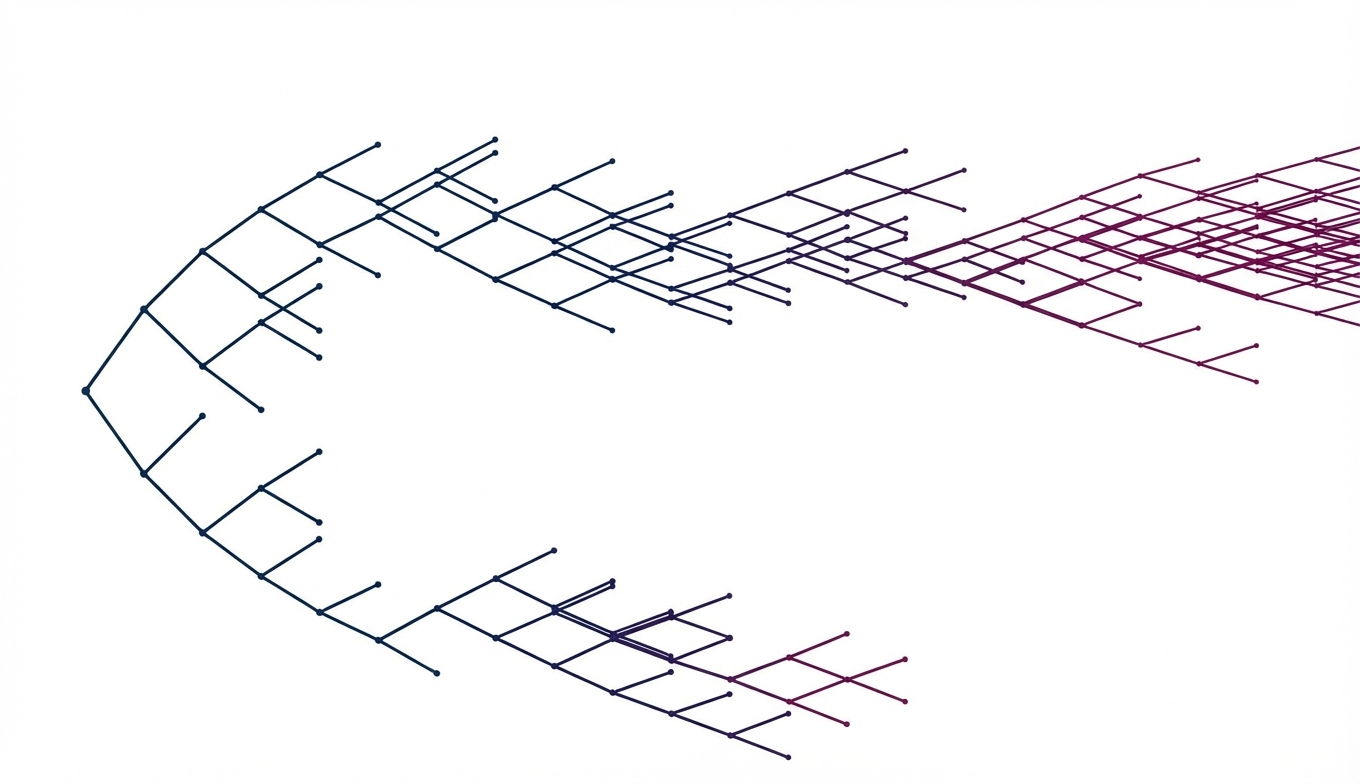
\includegraphics[width=0.78\textwidth]{figures/IMG_ch3/simpleGWvis.png}\\[6pt]
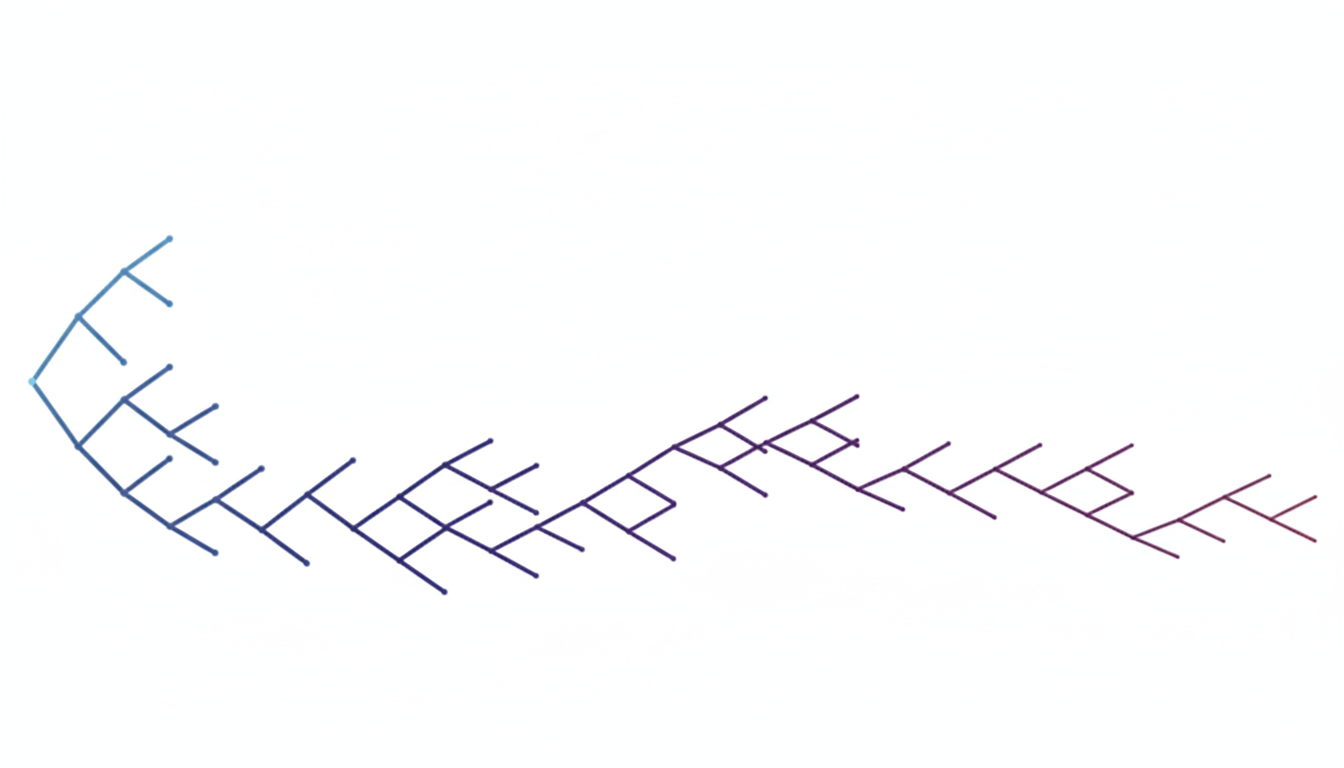
\includegraphics[width=0.78\textwidth]{figures/IMG_ch3/subGWvis.png}
\caption{Realisations of the simple Galton--Watson process, drawn as genealogies with generation increasing to the right. Top: supercritical, \(p=0.58\); the number of lines grows without bound. Bottom: subcritical, \(p=0.47\); the tree terminates. Colour encodes generation number.}
\label{fig:gwvis}
\end{figure}

The offspring \pgf{} is
\begin{equation}
\label{eq:pgfbinary}
\phi(z) = p z^2 + (1-p),
\end{equation}
so that \cref{iterPGF} becomes
\begin{equation}
\label{unIter}
u_{n+1} = p\,u_n^2 + 1-p .
\end{equation}
If the founder dies at the first step (probability \(1-p\)), extinction has already occurred. If it divides (probability \(p\)), extinction by generation \(n+1\) requires each of the two daughter lineages to die out within \(n\) generations, which has probability \(u_n^2\).

It is convenient to work with the survival probability
\begin{equation*}
S_n = 1-u_n = \pr{\zz_n>0}.
\end{equation*}
Substituting \(u_n=1-S_n\) into \cref{unIter} yields
\begin{equation}
\label{SnIter}
S_{n+1} = 2p S_n - p S_n^2,\qquad S_0 = 1.
\end{equation}
Because extinction is irreversible, \(u_n\) is non-decreasing and bounded by \(1\), so \(S_n\) is non-increasing and bounded below by \(0\), and therefore converges to some \(S_\infty\in[0,1]\).

\subsection{Certainty of extinction}
\label{sec:certainty}

Any limit of \cref{SnIter} must be a fixed point. Setting \(S_{n+1}=S_n=S_\infty\),
\begin{equation*}
S_\infty = 2p S_\infty - p S_\infty^2
\qquad\Longleftrightarrow\qquad
p\,S_\infty\bigl(S_\infty + \tfrac1p - 2\bigr) = 0,
\end{equation*}
with roots
\begin{equation*}
S_\infty = 0
\qquad\text{and}\qquad
S_\infty = \frac{2p-1}{p}.
\end{equation*}
For \(p<\tfrac12\) the second root is negative and inadmissible, so \(S_\infty=0\) and extinction is certain. At \(p=\tfrac12\) the roots coincide at the origin and extinction remains certain. For \(p>\tfrac12\) the positive root \(S_\infty=(2p-1)/p\) is attained: survival forever has positive probability. \Cref{fig:phase_transition} displays the transition.

\begin{figure}[htbp]
    \centering
    \begin{subfigure}[b]{0.31\textwidth}
        \centering
        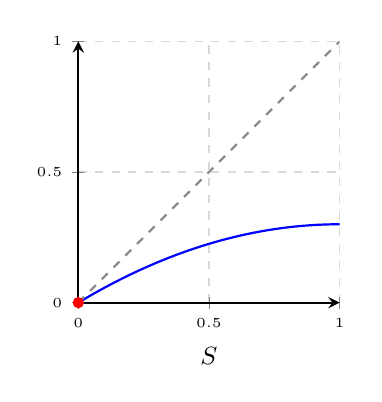
\begin{tikzpicture}
            \begin{axis}[myplotstyle]
                \addplot[blue, thick] {2*0.3*x - 0.3*x^2};
                \addplot[black!45, dashed] {x};
                \addplot[only marks, mark=*, red, mark size=1.6pt] coordinates {(0,0)};
            \end{axis}
        \end{tikzpicture}
        \caption{Subcritical (\(p = 0.3\))}
    \end{subfigure}
    \hfill
    \begin{subfigure}[b]{0.31\textwidth}
        \centering
        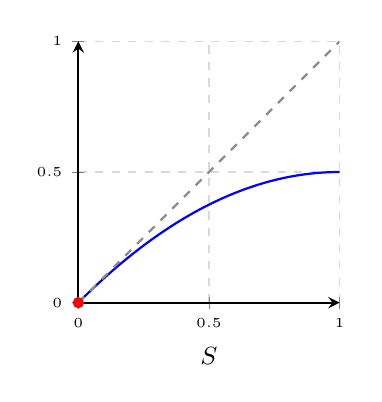
\begin{tikzpicture}
            \begin{axis}[myplotstyle]
                \addplot[blue, thick] {2*0.5*x - 0.5*x^2};
                \addplot[black!45, dashed] {x};
                \addplot[only marks, mark=*, red, mark size=1.6pt] coordinates {(0,0)};
            \end{axis}
        \end{tikzpicture}
        \caption{Critical (\(p = 0.5\))}
    \end{subfigure}
    \hfill
    \begin{subfigure}[b]{0.31\textwidth}
        \centering
        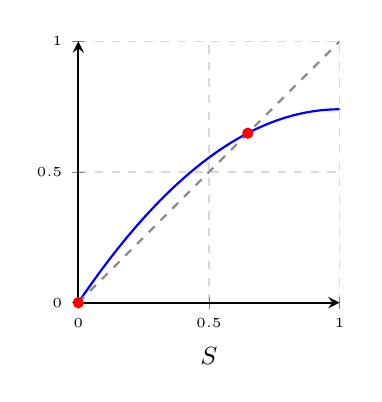
\begin{tikzpicture}
            \begin{axis}[myplotstyle]
                \addplot[blue, thick] {2*0.74*x - 0.74*x^2};
                \addplot[black!45, dashed] {x};
                \addplot[only marks, mark=*, red, mark size=1.6pt] coordinates {(0,0) (0.64865,0.64865)};
            \end{axis}
        \end{tikzpicture}
        \caption{Supercritical (\(p = 0.74\))}
    \end{subfigure}

    \vspace{10pt}
    \begin{subfigure}[b]{0.55\textwidth}
    \centering
    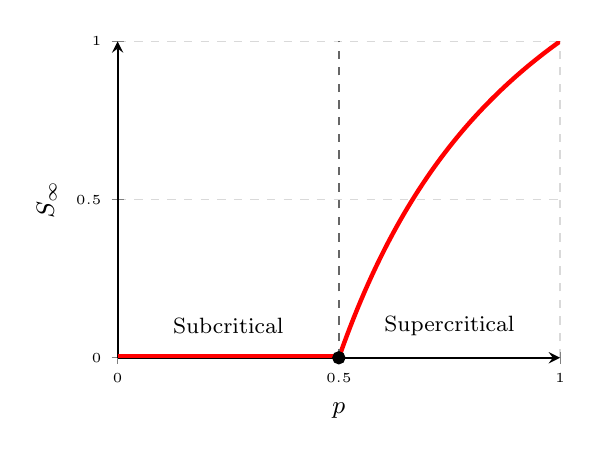
\begin{tikzpicture}
        \begin{axis}[
            width=7.2cm, height=5.6cm,
            axis lines=left,
            xlabel={$p$}, ylabel={$S_\infty$},
            xmin=0, xmax=1, ymin=0, ymax=1,
            xtick={0,0.5,1}, ytick={0,0.5,1},
            grid=major, grid style={dashed, gray!30}, thick,
            label style={font=\small}, tick label style={font=\tiny}
        ]
            \addplot[red, ultra thick, domain=0:0.5] {0.004};
            \addplot[red, ultra thick, domain=0.5:1, samples=120] {(2*x-1)/x};
            \draw[dashed, black!60] (axis cs:0.5,0) -- (axis cs:0.5,1);
            \node[font=\footnotesize] at (axis cs:0.25, 0.10) {Subcritical};
            \node[font=\footnotesize] at (axis cs:0.75, 0.10) {Supercritical};
            \addplot[only marks, mark=*, mark size=2pt, black] coordinates {(0.5,0)};
        \end{axis}
    \end{tikzpicture}
    \caption{The transition in $S_\infty$}
    \end{subfigure}

    \caption{Steady states of the survival recursion \cref{SnIter}. Panels (a)--(c) show the map \(S\mapsto 2pS-pS^{2}\) (blue) against the diagonal (dashed); fixed points are the intersections, marked in red. Below and at criticality the origin is the only fixed point in \([0,1]\), and it is attracting. For \(p>\tfrac12\) a stable positive fixed point \(S_\infty=(2p-1)/p\) separates from the origin, traced in panel~(d).}
    \label{fig:phase_transition}
\end{figure}

\subsection{The critical case: a power law and an infinite expected lifetime}
\label{sec:criticalcase}

At \(p=\tfrac12\) one has \(\mean{\zz_n}=1\) for every \(n\), yet extinction is certain. The reconciliation is that the expected lifetime is infinite: rare trajectories survive for very long times and become very large, at precisely the rate needed to hold the mean at one. The same calculation supplies the asymptotics of \(S_n\) used in \cref{sec:Ap}.

Let \(T=\inf\{n:\zz_n=0\}\) be the extinction time. Writing \(T\) as a sum of indicators and exchanging sum and expectation (all terms non-negative),
\begin{equation}
\label{eq:ETsumSn}
\mean{T} = \sum_{n=0}^{\infty}\pr{T>n} = \sum_{n=0}^{\infty}S_n .
\end{equation}
At \(p=\tfrac12\), \cref{SnIter} becomes \(S_{n+1}=S_n-\tfrac12 S_n^2\), or
\begin{equation*}
S_{n+1}-S_n = -\tfrac12 S_n^2 .
\end{equation*}
For large \(n\) the unit step is small relative to the scale on which \(S_n\) varies, and the left-hand side is well approximated by a derivative:
\begin{equation*}
\frac{\dd S}{\dd n} = -\tfrac12 S^2,
\qquad
S(n) = \frac{2}{n + \text{const}}.
\end{equation*}
Hence
\begin{equation}
\label{twoovrn_sn}
S_n \sim \frac{2}{n}\qquad (n\to\infty),
\end{equation}
confirmed by the simulations of \cref{fig:power_law}(a). Substituting into \cref{eq:ETsumSn}, the tail of the sum behaves like twice the harmonic series and diverges. Thus \(\mean{T}=\infty\): the expected lifetime of the critical process is infinite even though extinction occurs almost surely.

\begin{figure}[H]
    \centering
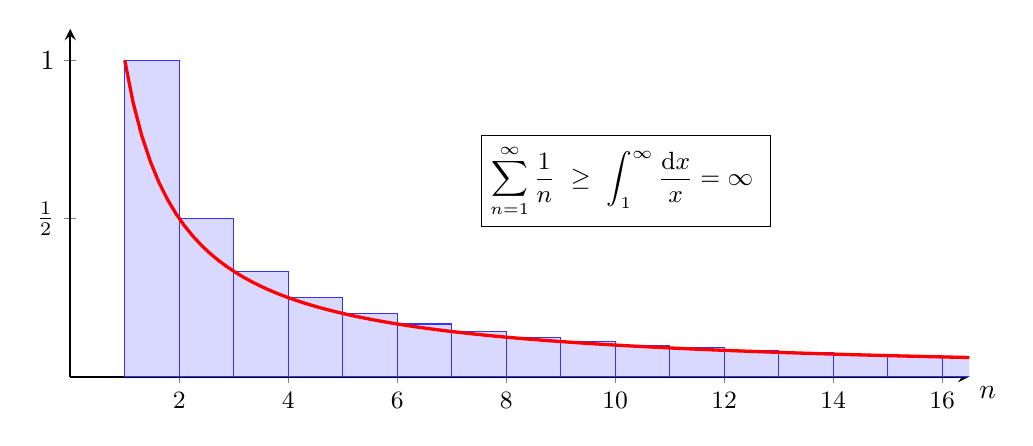
\begin{tikzpicture}
    \begin{axis}[
        axis lines = middle,
        xmin = 0, xmax = 16.5, ymin = 0, ymax = 1.1,
        xlabel = {$n$},
        xtick = {2,4,6,8,10,12,14,16},
        ytick = {0.5, 1}, yticklabels = {$\frac{1}{2}$, $1$},
        axis line style = {thick},
        width = 13cm, height = 6cm,
        every axis x label/.style={at={(current axis.right of origin)}, anchor=north west},
        xticklabel style={font=\small},
    ]
        \addplot[fill=blue!15, draw=blue!80, ybar interval, samples at={1,2,...,17}] {1/x} \closedcycle;
        \addplot[red, domain=1:16.5, samples=100, very thick] {1/x};
        \node[draw, fill=white, align=left, font=\small] at (axis cs: 10.2, 0.62) {
            $\displaystyle \sum_{n=1}^{\infty} \frac{1}{n} \ \ge\ \int_{1}^{\infty} \frac{\dd x}{x} = \infty$
        };
    \end{axis}
\end{tikzpicture}
\caption{Divergence of the harmonic series. Each blue rectangle has area \(1/n\) and contains the region under the curve \(1/x\) on \([n,n+1]\). Because \(S_n\sim 2/n\) at criticality, the same divergence carries over to \(\mean{T}=\sum_n S_n\).}
\label{fig:harmonic}
\end{figure}

\begin{figure}[ht]
    \centering
    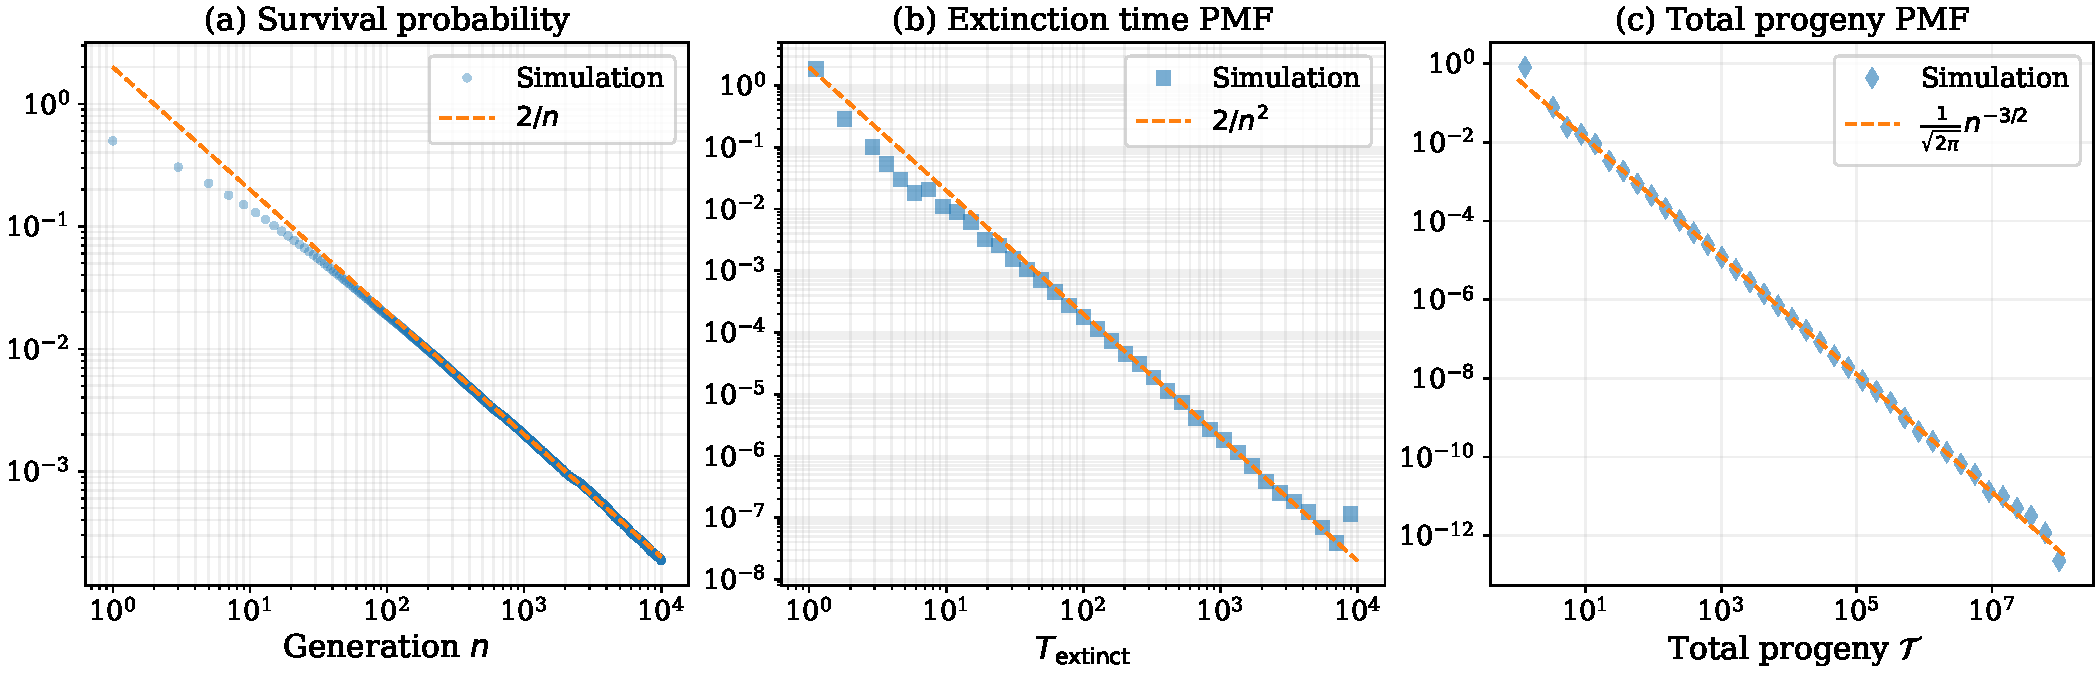
\includegraphics[width=0.98\textwidth]{figures/IMG_ch3/power_law_fixed.pdf}
    \caption{Power-law behaviour in the critical Galton--Watson process (\(p=0.5\)), from \(10^6\) realisations.
    (a) Survival probability \(S_n=\pr{\zz_n>0}\), showing \(S_n \sim 2/n\).
    (b) Probability mass function of the extinction time \(T\), with heavy tail \(\pr{T = n}\sim 2/n^{2}\).
    (c) Probability mass function of the total progeny \(\mathcal{T} = \sum_{k\ge0}\zz_k\), with the classical critical asymptotic \(\pr{\mathcal{T}=n}\sim n^{-3/2}\).}
    \label{fig:power_law}
\end{figure}

\FloatBarrier

\section{The limiting conditional distribution}
\label{sec:qsd}

When absorption is inevitable --- as it is for \(p<\tfrac12\) --- the unconditional process eventually sits at extinction. Before that happens, however, the law of the population \emph{conditional on not yet being extinct} may settle to a time-independent distribution. That limiting conditional law is the quasi-stationary, or Yaglom, distribution \cite{Yaglom1947,Athreya1972}. This section establishes its first two moments for the binary Galton--Watson process.

\subsection{Late-time survival probability}
\label{sec:lateS}

Everything follows from the decay of \(S_n\). For \(p<\tfrac12\), death is more likely than division at each step, \(S_n\to0\), and the quadratic term in
\begin{equation*}
S_{n+1} = 2pS_n - pS_n^2
\end{equation*}
becomes negligible relative to the linear term. The recursion is then well approximated by
\begin{equation}
\label{attenuated}
S_{n+1} \approx 2p\,S_n,
\end{equation}
and at late times
\begin{equation}
\label{lateS}
S_n \sim A(p)\,(2p)^n \qquad (n\to\infty),
\qquad
A(p) = \lim_{n\to\infty}\frac{S_n}{(2p)^n}.
\end{equation}
The constant \(A(p)\) accumulates the effect of the quadratic correction over the early generations, before the linear regime takes hold. The limit exists, is finite, and is strictly positive for \(p\in[0,\tfrac12)\); existence via an infinite product is proved in \cref{sec:product}, and \cref{sec:Abounds} places \(A(p)\) in \((0,\tfrac12]\).

\begin{remark}
Relation \cref{lateS} is an asymptotic equivalence, not an identity for each \(n\). One must not write \(\lim_n S_n = A(p)(2p)^n\): the right-hand side still depends on \(n\). What converges is the ratio \(S_n/(2p)^n\).
\end{remark}

\subsection{Mean}
\label{sec:condmean}

Decompose the expected size into extinct and surviving contributions:
\begin{equation*}
\mean{\zz_n}
= \pr{\zz_n = 0}\,\cancelto{0}{\mean{\zz_n\mid \zz_n = 0}}
+ \pr{\zz_n > 0}\,\mean{\zz_n \mid \zz_n > 0}.
\end{equation*}
The first term vanishes, so with \(\pr{\zz_n>0}=S_n\) and \(\mean{\zz_n}=(2p)^n\),
\begin{equation}
\label{eq:condmeandef}
\mean{\zz_n \mid \zz_n > 0} = \frac{\mean{\zz_n}}{S_n} = \frac{(2p)^n}{S_n}.
\end{equation}
Inserting \cref{lateS},
\begin{equation}
\label{eq:qsmean}
\mean{\zz_n \mid \zz_n > 0} \;\xrightarrow[n\to\infty]{}\; \frac{1}{A(p)}.
\end{equation}
The geometric factors cancel exactly. At late times the surviving population has constant expected size \(1/A(p)\), the \emph{quasi-stationary mean}.

\Cref{fig:condmean} shows the approach to the plateau. The closer \(p\) is to \(\tfrac12\), the higher the plateau and the longer the wait --- the near-critical difficulty that \cref{sec:Ap} must confront.

\begin{figure}[ht]
\centering
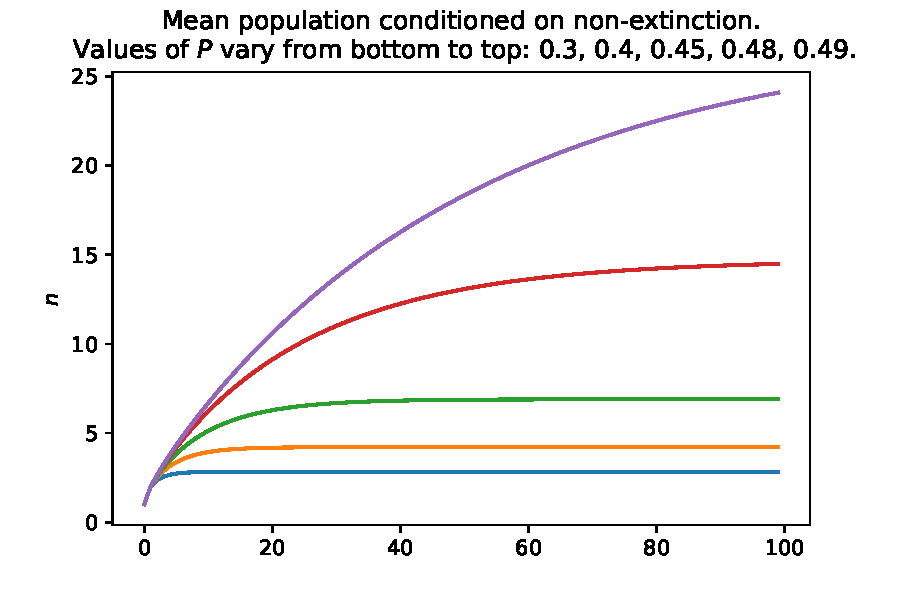
\includegraphics[width=0.78\textwidth]{figures/IMG_ch3/conditionalMean.pdf}
\caption{Conditional mean \((2p)^n/S_n\) against generation \(n\), with \(S_n\) from iterating \cref{SnIter}. From bottom to top, \(p = 0.3,\,0.4,\,0.45,\,0.48,\,0.49\). Each curve approaches \(1/A(p)\); approximate plateaus are \(2.825\), \(4.208\), \(6.893\), \(14.703\) and \(27.476\) (computed as in \cref{sec:practical}). Near \(p=0.49\) convergence is visibly slow.}
\label{fig:condmean}
\end{figure}

\subsection{Variance}
\label{sec:variance}

Stabilisation of the conditional mean is not enough for quasi-stationarity of the full law; the second moment is needed.

\subsubsection{The second moment \(\mean{\zz_n^2}\)}

For a random variable \(\xx\) the moment generating function is \(\mean{\ee^{t\xx}}\), which may be written through the \pgf{} as \(\phi(\ee^t)\). For the binary offspring law \cref{eq:pgfbinary},
\begin{equation}
\label{mgf1}
M_1(t) = \phi_1(\ee^t) = p\,\ee^{2t} + (1-p),
\end{equation}
the subscript \(1\) marking generation \(n=1\). Moments follow from
\begin{equation}
\label{mgf2}
\mean{\zz_n^r} = \frac{\dd^r}{\dd t^r}M_n(t)\bigg|_{t=0}.
\end{equation}
Differentiating \cref{mgf1} twice at \(t=0\) gives \(\mean{\zz_1^2}=4p\). To reach generation \(n\), recall that the \(n\)-step \pgf{} is the \(n\)-fold composition of \(\phi_1\), so
\begin{equation*}
M_n(t) = \phi_1\lrbq{\phi_1\lrbq{\dots\phi_1\lrbq{\ee^t}}}.
\end{equation*}
Differentiating once by the chain rule,
\begin{equation}
\label{dmgf1}
M_n'(t) = \phi_1'\lrbq{\phi_{n-1}\lrbq{\ee^t}}\cdot\phi_1'\lrbq{\phi_{n-2}\lrbq{\ee^t}}\cdots\phi_1'\lrbq{\ee^t}\cdot\ee^t .
\end{equation}
Since \(\phi_1'(z)=2pz\), this collapses to
\begin{equation}
\label{dmgf2}
M_n'(t) = (2p)^n\cdot M_{n-1}(t)\cdot M_{n-2}(t)\cdots M_1(t)\cdot\ee^{2t}.
\end{equation}
At \(t=0\) every factor equals \(1\). Differentiating the product \cref{dmgf2} produces a sum of terms in which exactly one factor is differentiated:
\begin{align*}
M_n''(t) = (2p)^n\bigg[\,&M_{n-1}'(t)\cdot M_{n-2}(t)\cdots M_1(t)\cdot\ee^{2t}\\
+ &M_{n-1}(t)\cdot M_{n-2}'(t)\cdots M_1(t)\cdot\ee^{2t}\\
&\hspace{60pt}\vdots\\
+ &M_{n-1}(t)\cdot M_{n-2}(t)\cdots M_1'(t)\cdot\ee^{2t}\\
+ &M_{n-1}(t)\cdot M_{n-2}(t)\cdots M_1(t)\cdot 2\ee^{2t}\,\bigg].
\end{align*}
Evaluating at \(t=0\) and using \(M_k'(0)=(2p)^k\) yields
\begin{equation*}
M_n''(0) = (2p)^n\lrbs{\sum_{i=0}^{n-1}(2p)^i + 1}.
\end{equation*}
Summing the geometric series and rearranging,
\begin{equation}
\label{secondMoment}
\mean{\zz_n^2} = (2p)^n\lrb{1 + \frac{1}{1-2p}} - (2p)^{2n}\lrb{\frac{1}{1-2p}},
\end{equation}
which recovers \(\mean{\zz_1^2}=4p\) at \(n=1\).

\subsubsection{Late-time variance}

From \(\mathrm{Var}(\zz_n)=\mean{\zz_n^2}-\mean{\zz_n}^2\) and \cref{secondMoment}, for \(2p<1\) the leading large-\(n\) term of the unconditional variance is of order \((2p)^n\). Conditional moments, however, are formed by dividing by \(S_n\). Using \cref{lateS},
\begin{align*}
\mean{\zz_n^2\mid \zz_n\neq0} &\xrightarrow{n\to\infty}
\frac{1}{A}\lrb{1+\frac{1}{1-2p}},\\[4pt]
\mean{\zz_n\mid \zz_n\neq0} &\xrightarrow{n\to\infty}
\frac{1}{A},
\end{align*}
so the conditional variance tends to a finite constant:
\begin{equation}
\label{eq:condvar}
\mathrm{Var}(\zz_n\mid \zz_n\neq0) \;\longrightarrow\; \frac{1}{A}\lrb{1+\frac{1}{1-2p}} - \frac{1}{A^2}.
\end{equation}
Both conditional moments are expressed entirely in terms of \(p\) and the single unknown \(A(p)\). Higher moments settle by the same mechanism, yielding the full quasi-stationary distribution. Everything now turns on that constant.

\subsection{A continuum view of the survival recursion}
\label{sec:riccati}

Write \(r=1-2p\) for the distance from criticality. The recursion \cref{SnIter} rearranges to
\begin{equation}
\label{eq:Sdiff}
S_{n+1}-S_n = -r S_n - p S_n^2 .
\end{equation}
For large \(n\) the left-hand side is well approximated by a derivative, giving the Riccati equation
\begin{equation}
\label{eq:riccati}
\frac{\dd S}{\dd n} = -r S - p S^2 .
\end{equation}
The substitution \(u=1/S\) linearises it to \(u'=ru+p\), with solution
\begin{equation}
\label{eq:riccatisol}
S(n) = \frac{r}{K r\,\ee^{rn} - p},
\end{equation}
\(K\) fixed by initial data. Setting \(r=0\) recovers the critical scaling \(S\sim2/n\); keeping \(r>0\) recovers geometric decay of the form \(S\sim A(2p)^n\). The integration constant \(K\) is determined by early generations where the continuum approximation fails --- which is another way of saying that it is \(A(p)\), and that no purely continuum argument will produce it. \Cref{sec:asymptotic} extracts what can still be obtained near criticality.

\FloatBarrier

\section{Survival of small populations}
\label{sec:small}

Return to the binary Galton--Watson process near criticality, with \(p\) and \(1-p\) each close to one half. A lineage dies at the first generation with probability about \(\tfrac12\). Conditional on dividing, both daughters fail at their first attempt with probability about \(\tfrac14\), so the chance of still being alive at generation two is only about \(0.375\):
\begin{equation*}
0.375 \approx \underbrace{(1-0.5)}_{\text{survive step 1}}\times\underbrace{(1-0.5\times0.5)}_{\text{survive step 2}} .
\end{equation*}
Iterating the \pgf{} gives the precise early values. With \(\phi(z)=pz^2+(1-p)\),
\begin{equation}
\label{ext}
u_{n+1} = p\,u_n^2 + 1-p ,
\qquad
S_{n+1} = 2pS_n - pS_n^2 ,
\end{equation}
started at \(u_0=0\), \(S_0=1\). At exact criticality the first four extinction probabilities are
\begin{equation*}
u_n = 0.500,\ 0.625,\ 0.695,\ 0.741\quad(3\ \text{s.f.}),
\end{equation*}
so survival decays quickly even just above criticality (\cref{fig:earlySn}).

\begin{figure}[ht]
\centering
  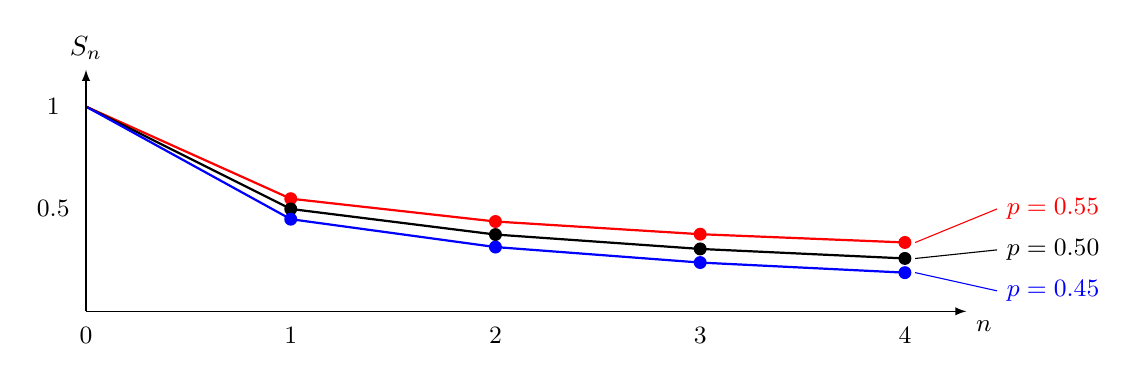
\begin{tikzpicture}[scale = 2.6]
    \foreach \x/\y/\color in {1/0.55/red, 2/0.4386250/red, 3/0.3766719/red, 4/0.336304/red,
                              1/0.5/black, 2/0.375/black, 3/0.3046875/black, 4/0.25827/black,
                              1/0.449999/blue, 2/0.313874/blue, 3/0.2381546/blue, 4/0.188816/blue}
      \fill[color=\color] (\x, \y) circle (0.9pt);
    \draw[red, thick] (0, 1) -- (1, 0.55) -- (2, 0.4386250) -- (3,0.3766719) -- (4,0.336304);
    \draw[black, thick] (0, 1)--(1,0.5) --  (2,0.375) -- (3,0.304687) -- (4,0.25827);
    \draw[blue, thick] (0, 1)--(1,0.449999)  --  (2,0.313874) -- (3,0.238154) -- (4,0.18881);
    \draw[-latex] (0,0) -- (4.3,0) node[below right, font=\small] {$n$};
    \draw[-latex] (0,0) -- (0,1.18) node[above] {$S_n$};
    \foreach \x/\lab in {0/0, 1/1, 2/2, 3/3, 4/4} \node[font=\small] at (\x, -0.12) {\lab};
    \foreach \y/\lab in {0.5/0.5, 1/1} \node[font=\small] at (-0.16, \y) {\lab};
    \draw[red,  thin] (4.05,0.336) -- (4.45,0.50);
    \draw[black,thin] (4.05,0.258) -- (4.45,0.30);
    \draw[blue, thin] (4.05,0.189) -- (4.45,0.10);
    \node[red,  font=\small, anchor=west] at (4.45, 0.50) {$p=0.55$};
    \node[black,font=\small, anchor=west] at (4.45, 0.30) {$p=0.50$};
    \node[blue, font=\small, anchor=west] at (4.45, 0.10) {$p=0.45$};
  \end{tikzpicture}
\caption{Survival probability over the first four generations from a single progenitor, from \cref{ext}. Even for \(p=0.55\) the early decay is steep; the three curves have barely separated by \(n=4\).}
\label{fig:earlySn}
\end{figure}

\subsection{An initial cohort of size \texorpdfstring{$k$}{k}}
\label{sec:cohort}

Now take \(\zz_0=k\): the process begins with a small founding group (for instance \(k=10\) pathogenic particles). Under supercritical growth the law of large numbers eventually stabilises the trajectory, but the founding phase is precisely where stochasticity dominates. The probability that at least one of the \(k\) independent lineages remains alive at generation \(n\) is
\begin{equation}
\label{eq:Snk}
S^{(k)}_n = 1 - \bigl({}_1u_n\bigr)^{k},
\end{equation}
where \({}_1u_n\) is the single-lineage extinction probability.

\begin{figure}[ht]
\centering
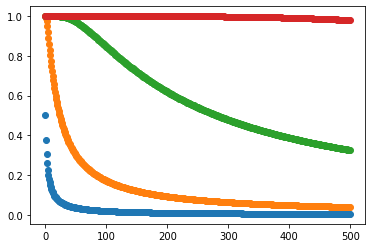
\includegraphics[width=0.56\textwidth]{figures/IMG_ch3/kvals.png}
\caption{Survival probability \(S^{(k)}_n\) from \cref{eq:Snk} out to \(500\) generations at exact criticality, \(p=0.5\), for \(k=1,10,100,1000\) (blue through to red). A larger founding cohort buys longevity, but at criticality every curve still tends to zero.}
\label{fig1}
\end{figure}

\begin{figure}[ht]
\centering
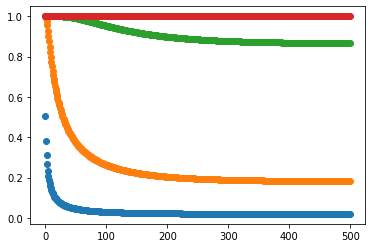
\includegraphics[width=0.45\textwidth]{figures/IMG_ch3/kvals505.png}
\hfill
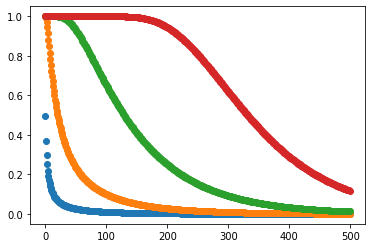
\includegraphics[width=0.45\textwidth]{figures/IMG_ch3/kvals495.png}
\caption{As \cref{fig1}, with \(p\) displaced slightly from criticality: \(p=0.505\) (left, supercritical) and \(p=0.495\) (right, subcritical). A half-percent shift separates curves that were nearly coincident at criticality.}
\label{fig2}
\end{figure}

\Cref{fig1,fig2} show \(S_n^{(k)}\) through \(500\) generations. The benefit of a larger inoculum is acutely sensitive to which side of \(\tfrac12\) the process sits on.

\subsection{An aside on early replication}
\label{sec:earlyrep}

The same conditioning effect appears in a different setting: the longevity and diversity of phylogenetic clades. Clades that persist to the present tend to show elevated early origination rates in the fossil record. Budd and Mann \cite{Budd2018} argue that this need not reflect a biological slowdown later on: if one simulates many homogeneous birth--death processes and retains only those still alive at a large observation time, the retained set is automatically enriched for early rapid growth --- the \emph{push of the past}. That is the conditioning of \cref{sec:qsd} read the other way: there one conditions a subcritical process on survival and finds a finite quasi-stationary mean; here one conditions a critical or supercritical process on survival to the present and finds inflated early growth.

On the pathogenic side the parallel suggests that securing a high probability of early replication may matter disproportionately, even if later per-capita rates are less favourable. \Cref{fig:earlySn} makes the point quantitatively: the first few generations concentrate most of the extinction risk.

\subsection{Discrete birth--death--catastrophe}
\label{sec:bdc}

Until catastrophe fires, a discrete-time birth--death--catastrophe process behaves, for the purpose of limiting conditional laws given non-extinction and non-rupture, like the Galton--Watson model above. Whether a quasi-stationary distribution survives when one conditions only on avoiding both death and catastrophe is a separate question, best settled by simulation for a given rate structure. In any case the probability of avoiding catastrophe is needed as a building block. Full continuous-time birth--death--catastrophe analysis --- means, variances, burst sizes, and quasi-stationarity under rupture --- is developed in Chapters~3--5; here we record the discrete survival formulae from the seed material and define the continuous rates.

\subsubsection*{Probability of rupture at step \texorpdfstring{$n$}{n}}

Let \(\kappa\) be the probability that a given individual initiates catastrophe at a step. A cohort of size \(N\) fails to rupture with probability \((1-\kappa)^N\).

In the birth-and-catastrophe case with no death, the living census is deterministic: from a single progenitor the population doubles at each step prior to catastrophe. Rupture occurs at generation \(n\) with probability
\begin{equation*}
1-(1-\kappa)^{2^{\,n-1}},
\end{equation*}
one minus the probability that none of the \(2^{n-1}\) individuals present triggered it.

\subsubsection*{Probability of process survival}

Still without death, let \(S_n\) be the probability that the process reaches generation \(n\) without catastrophe. Then \(S_0=1\), \(S_1=1-\kappa\), and survival to step \(2\) requires the founder and both offspring to avoid rupture:
\begin{equation*}
S_2 = (1-\kappa)(1-\kappa)^2 .
\end{equation*}
In general
\begin{equation}
\label{eq:bdcS}
S_n = \prod_{i=0}^{n-1}(1-\kappa)^{2^i} = (1-\kappa)^{2^n-1}.
\end{equation}

\subsubsection*{Death included}

Once death is allowed, the living census is random. Replacing the random count by its mean in the survival product,
\begin{equation}
\label{eq:bdcguess}
S_n \overset{?}{=} (1-\kappa)^{\sum_{i=0}^{n-1}\mean{\xx_i}} ,
\end{equation}
is not an identity. The map \(N\mapsto(1-\kappa)^N\) is convex, so Jensen's inequality gives \(\mean{(1-\kappa)^{\xx_i}}\ge(1-\kappa)^{\mean{\xx_i}}\): the mean underestimates the chance of passing a step. Surviving one step is also informative about a smaller population, which raises the chance of surviving the next. Both effects act in the same direction, so \cref{eq:bdcguess} is better read as a lower bound than as an equality.

\subsubsection*{Continuous-time BDC (definition and forward pointer)}

In continuous time, a single-type birth--death--catastrophe process on \(\{0,1,2,\dots\}\) with per-capita birth rate \(\lambda\), death rate \(\mu\), and catastrophe rate \(\delta\) has transitions
\begin{equation}
\label{eq:bdc-ct-rates}
i \to i+1 \text{ at rate } i\lambda,\qquad
i \to i-1 \text{ at rate } i\mu,\qquad
i \to R \text{ at rate } i\delta,
\end{equation}
where \(R\) is an absorbing rupture state. The process encodes intracellular load growth with load-dependent risk of host-cell rupture. Means, generating-function PDEs, burst-size distributions, and quasi-stationary structure for this model (and its two-type extensions) are developed in Chapters~3--5; the present chapter supplies the branching, quasi-stationary, and characteristics tools those chapters use.

\subsection{Continuous-time birth--death}
\label{sec:cts}

The discrete constant \(A(p)\) has no elementary closed form (\cref{sec:Ap}). Its continuous-time counterpart does, and the comparison is informative.

For the linear birth--death process with per-capita rates \(\lambda\) and \(\mu\), started from \(N\) individuals, the extinction probability is \cite{Allen2010}
\begin{equation}
\label{eq:p0t}
p_0(t) = \begin{cases}
\lrb{\dfrac{\mu - \mu \ee^{(\mu-\lambda)t}}{\lambda - \mu \ee^{(\mu-\lambda)t}}}^{N}, & \lambda \neq \mu,\\[12pt]
\lrb{\dfrac{\lambda t}{1+\lambda t}}^{N}, & \lambda = \mu,
\end{cases}
\end{equation}
and \(S^{(N)}(t)=1-p_0(t)\).

\subsubsection*{Limiting mean conditioned on non-extinction}

When \(\mu>\lambda\) (subcritical), the conditional mean settles. With \(N=1\),
\begin{equation*}
\mean{\xt}=\ee^{(\lambda-\mu)t},
\qquad
S(t)=\frac{\lambda-\mu}{\lambda - \mu\ee^{(\mu-\lambda)t}},
\end{equation*}
so
\begin{equation*}
\mean{\xt \mid \xt > 0} = \frac{\lambda\ee^{(\lambda-\mu)t} - \mu}{\lambda-\mu}
\xrightarrow{t\to\infty}
\frac{\mu}{\mu-\lambda}.
\end{equation*}
Writing \(p=\lambda/(\lambda+\mu)\) so that \(\lambda/\mu=p/(1-p)\),
\begin{equation}
\label{eq:Acts}
A_{\text{c}}(p) = \frac{1-2p}{1-p},
\qquad
\frac{1}{A_{\text{c}}} = \frac{1-p}{1-2p}.
\end{equation}
The subscript marks the continuous-time constant, distinguished from the discrete \(A(p)\) of \cref{lateS}.

\begin{figure}[ht]
\centering
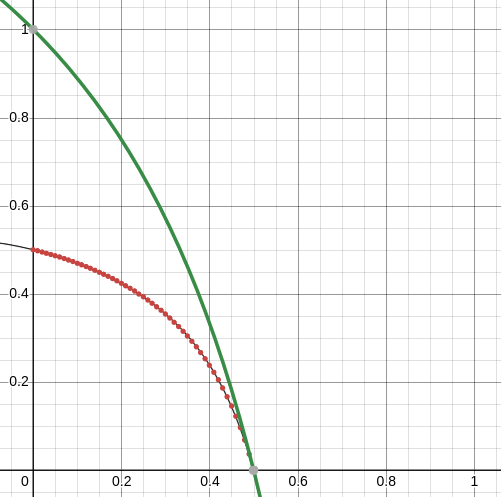
\includegraphics[width=0.5\textwidth]{figures/IMG_ch3/dtctA.png}
\caption{Continuous-time \(A_{\text{c}}(p)=(1-2p)/(1-p)\) (green) against high-precision numerical values of discrete \(A(p)\) (red). Both vanish at \(p=\tfrac12\), but at \(p=0\) the continuous curve starts at \(1\) and the discrete one at \(\tfrac12\); they are not related by a constant factor. The black curve is a symbolic-regression candidate from \cref{sec:GA}; it tracks the points closely but is not exact. \Cref{sec:compare} accounts for the discrepancy.}
\label{fig:dtct}
\end{figure}

\Cref{fig:dtct} raises the natural question: why do the curves start at different heights yet meet near criticality? \Cref{sec:compare} answers once the series representation of \(A(p)\) is available.

\FloatBarrier

\section{The constant \texorpdfstring{$A(p)$}{A(p)}}
\label{sec:Ap}

Everything in \cref{sec:qsd} reduced to the single constant
\begin{equation}
\label{eq:Ap-def}
A(p) = \lim_{n\to\infty}\frac{S_n}{(2p)^n},\qquad p\in[0,\tfrac12),
\end{equation}
whose reciprocal is the quasi-stationary mean. Approximate values are obtained by iterating \(S_{n+1}=f(S_n)\) until near stationarity and forming \(S_n/(2p)^n\). Over most of the interval this is reliable; it fails as \(p\to\tfrac12^-\), because the number of generations needed grows without bound.

No formula in elementary functions is known for \(A(p)\). This section records what is known: an exact infinite product (\cref{sec:product}); an exact series with two-sided bounds that pin \(A(p)\) between the continuous-time constant of \cref{sec:cts} and twice that bound's companion (\cref{sec:Abounds}); the near-critical asymptotic \(A(p)\sim2(1-2p)\) (\cref{sec:asymptotic}); a resolution of the discrete--continuous discrepancy (\cref{sec:compare}); an account of symbolic-regression searches (\cref{sec:GA}); and the dynamical argument explaining why a closed form is not to be expected (\cref{sec:koenigs}). \Cref{sec:practical} summarises practical computation.

\subsection{An infinite-product representation}
\label{sec:product}

Start from the survival map \(S_{n+1}=2pS_n-pS_n^2\), \(S_0=1\), and set \(S_n=2w_n\). Then
\begin{equation}
\label{eq:logistic}
w_{n+1} = 2p\,w_n(1-w_n) = r\,w_n(1-w_n),\qquad r = 2p,\ \ w_0 = \tfrac12 ,
\end{equation}
which is the logistic map. The celebrated period-doubling cascade as \(r\) increases from \(0\) to \(4\) is recalled in \cref{fig:period_double}; the subcritical branching window is \(r\in[0,1)\), at the extreme left of that picture, where the origin is globally attracting. That this corner of the logistic family is nevertheless enough to obstruct a closed form is the content of \cref{sec:koenigs}.

\begin{figure}[ht]
    \centering
    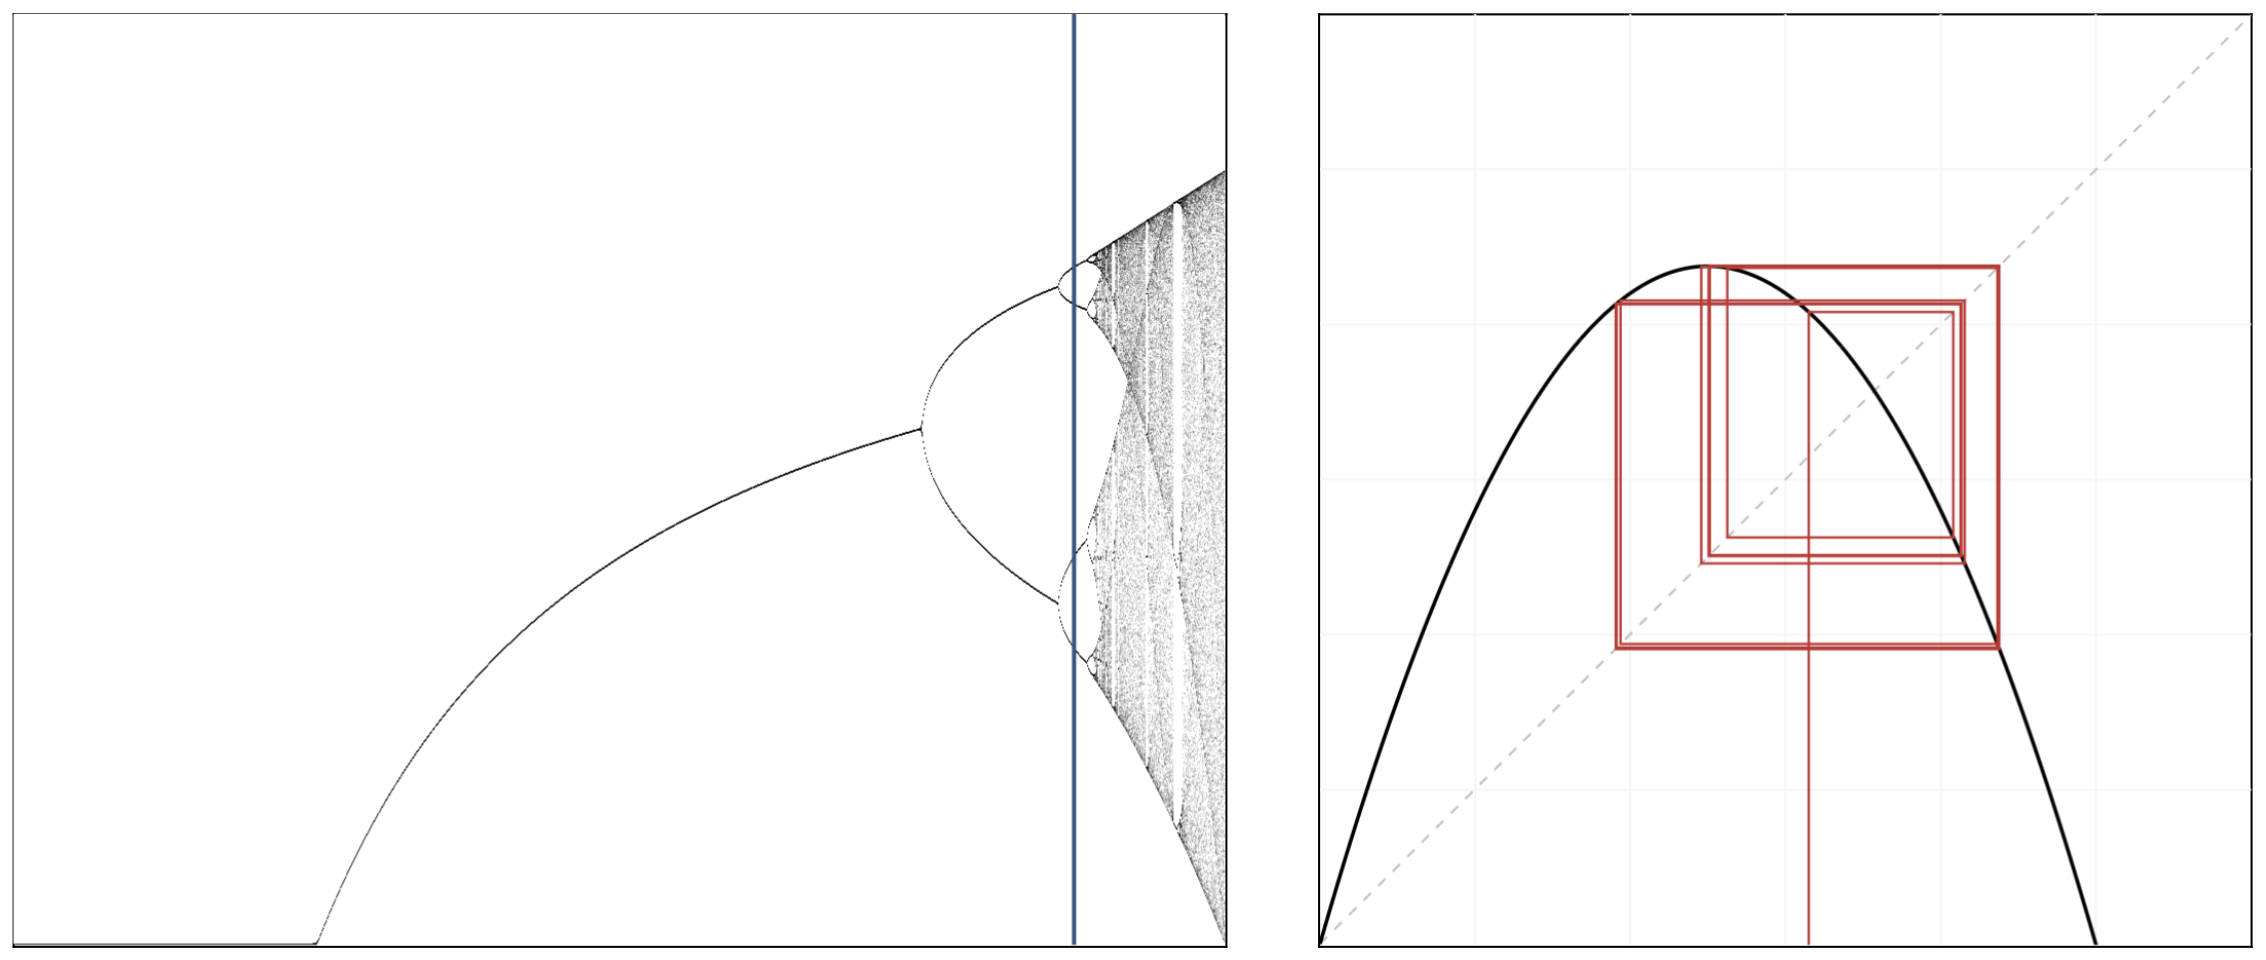
\includegraphics[width=0.86\textwidth]{figures/IMG_ch3/period_double.png}
    \caption{Bifurcation diagram of the logistic map \(w\mapsto rw(1-w)\). The regime relevant to subcritical branching is \(r=2p\in[0,1)\), off the left-hand edge, where the dynamics are as simple as they can be.}
    \label{fig:period_double}
\end{figure}

In terms of \(w\),
\begin{equation}
\label{eq:Aw}
A(p) = 2\lim_{n\to\infty}\frac{w_n}{r^n}.
\end{equation}
Any sequence admits a telescoping product representation. Applying it to \(x_n=w_n/r^n\) yields ratios
\begin{equation*}
\frac{x_{k+1}}{x_k}=1-w_k,
\end{equation*}
and therefore
\begin{equation}
\label{eq:prodFormula}
A(p) = \frac12\prod_{k=1}^{\infty}\lrb{1-w_k} = \frac12\prod_{k=1}^{\infty}\lrb{1-\frac{S_k}{2}}.
\end{equation}

\subsubsection*{Convergence}

For \(0<w_k<1\) the product \(\prod_{k\ge1}(1-w_k)\) converges to a strictly positive limit if and only if \(\sum w_k<\infty\). From \cref{eq:logistic} with \(0<r<1\) one has \(w_{n+1}<rw_n\), so \(w_n\le w_0 r^n\). The bound is summable, the product converges, and the limit \cref{eq:Ap-def} exists in \((0,\tfrac12)\) for \(p\in(0,\tfrac12)\).

\subsubsection*{Is this an advance?}

Only a modest one. Partial products of \cref{eq:prodFormula} are monotone decreasing and supply rigorous upper bounds on \(A(p)\), which the raw ratio \(S_n/(2p)^n\) does not. Computing the factors still requires iterating the nonlinear map, so the near-critical difficulty remains. The product does, however, open a route to the sharper series of the next subsection.

\subsection{An exact series and two-sided bounds}
\label{sec:Abounds}

Write \(r=2p\) and \(S_{n+1}=rS_n\bigl(1-S_n/2\bigr)\). Define \(v_n=r^n/S_n\), so that \(v_n\to1/A(p)\). Then
\begin{equation*}
v_{n+1}-v_n = \frac{r^n}{2-S_n}.
\end{equation*}
Summing from \(v_0=1\) yields an exact representation of the quasi-stationary mean.

\begin{proposition}[Series representation]
\label{prop:series}
For \(p\in[0,\tfrac12)\), with \(S_n\) generated by \cref{SnIter},
\begin{equation}
\label{eq:Aseries}
\frac{1}{A(p)} = 1 + \sum_{n=0}^{\infty}\frac{(2p)^n}{2-S_n}.
\end{equation}
\end{proposition}

Unlike the product, this form isolates geometric decay in a factor independent of the early nonlinear dynamics; the whole of the nonlinearity sits in the bounded denominator \(2-S_n\in[1,2)\). Bounding the denominator by its extremes and summing the resulting geometric series produces the following.

\begin{proposition}[Two-sided bounds]
\label{prop:bounds}
Write \(\varepsilon = 1-2p\). Then for \(p\in(0,\tfrac12)\)
\begin{equation}
\label{eq:Abounds}
\frac{\varepsilon}{1+\varepsilon} \;<\; A(p) \;<\; \frac{2\varepsilon}{1+2\varepsilon},
\end{equation}
equivalently
\begin{equation}
\label{eq:Aboundsexplicit}
\frac{1-2p}{2(1-p)} \;<\; A(p) \;<\; \frac{2(1-2p)}{3-4p}.
\end{equation}
The lower bound is exactly half the continuous-time constant of \cref{eq:Acts}:
\begin{equation}
\label{eq:halfAc}
A(p) > \tfrac12 A_{\text{c}}(p).
\end{equation}
\end{proposition}

\begin{proof}
Since \(0<S_n\le1\), one has \(\tfrac12 r^n < r^n/(2-S_n)\le r^n\) (equality on the right only at \(n=0\)). Summing and using \(\sum r^n=1/\varepsilon\) gives
\begin{equation*}
1+\frac{1}{2\varepsilon} \;<\; \frac{1}{A(p)} \;<\; 1+\frac{1}{\varepsilon},
\end{equation*}
and inversion produces \cref{eq:Abounds}. Substituting \(\varepsilon=1-2p\) gives \cref{eq:Aboundsexplicit}, whose lower bound equals \(\tfrac12 A_{\text{c}}(p)\).
\end{proof}

As \(p\to0\), \(\varepsilon\to1\) and the lower bound tends to \(\tfrac12\). Combined with the parity bound below, \(A(0^+)=\tfrac12\). As \(p\to\tfrac12^-\), the lower bound behaves like \(\varepsilon\) and the upper like \(2\varepsilon\); \cref{sec:asymptotic} shows that the upper bound is attained asymptotically. Thus \(A(p)\) runs from its lower bound at one end of the interval to its upper bound at the other, and no constant rescaling of \(A_{\text{c}}\) can reproduce it.

\begin{proposition}[Parity bound]
\label{prop:parity}
For the binary Galton--Watson process started from a single individual, \(A(p)\le\tfrac12\) for all \(p\in[0,\tfrac12)\), with equality approached as \(p\to0\).
\end{proposition}

\begin{proof}
Every individual leaves \(0\) or \(2\) offspring, so \(\zz_n\) is even for every \(n\ge1\). Conditional on survival, \(\zz_n\ge2\), hence \(\mean{\zz_n\mid \zz_n>0}\ge2\). Taking \(n\to\infty\) and using \cref{eq:qsmean} gives \(1/A(p)\ge2\). As \(p\to0\) the conditional population is \(2\) with probability tending to one, so the bound is attained in the limit.
\end{proof}

\begin{table}[ht]
\centering
\caption{The constant \(A(p)\) from the product \cref{eq:prodFormula} in high-precision arithmetic, against the bounds of \cref{prop:bounds} and the near-critical asymptotic \(2(1-2p)\). The last two columns give the quasi-stationary mean and the number of factors needed for full precision.}
\label{tab:Avals}
\begin{tabular}{ccccccr}
\toprule
$p$ & $\tfrac12 A_{\text{c}}(p)$ & $A(p)$ & $\dfrac{2(1-2p)}{3-4p}$ & $2(1-2p)$ & $1/A(p)$ & iterations\\
\midrule
0.05   & 0.473684 & 0.486180 & 0.642857 & 1.800000 & 2.0568 & 45 \\
0.1    & 0.444444 & 0.469382 & 0.615385 & 1.600000 & 2.1305 & 64 \\
0.2    & 0.375000 & 0.423895 & 0.545455 & 1.200000 & 2.3591 & 113 \\
0.3    & 0.285714 & 0.353967 & 0.444444 & 0.800000 & 2.8251 & 201 \\
0.4    & 0.166667 & 0.237647 & 0.285714 & 0.400000 & 4.2079 & 458 \\
0.45   & 0.090909 & 0.145069 & 0.166667 & 0.200000 & 6.8933 & 966 \\
0.48   & 0.038462 & 0.068011 & 0.074074 & 0.080000 & 14.7036 & 2\,473 \\
0.49   & 0.019608 & 0.036395 & 0.038462 & 0.040000 & 27.4764 & 4\,965 \\
0.499  & 0.001996 & 0.003944 & 0.003984 & 0.004000 & 253.519 & 48\,992 \\
0.4999 & 0.000200 & 0.000399 & 0.000400 & 0.000400 & 2504.65 & 478\,905 \\
\bottomrule
\end{tabular}
\end{table}

\subsection{Behaviour as \texorpdfstring{$p\to\tfrac12^-$}{p to 1/2}}
\label{sec:asymptotic}

The series \cref{eq:Aseries} delivers the near-critical asymptotic transparently. Fix \(\varepsilon=1-2p\) small. The summand \(r^n/(2-S_n)\) involves two scales: geometric decay on \(n\sim1/\varepsilon\), and survival \(S_n\) already near its critical law \(S_n\sim2/n\) over that range. For the overwhelming majority of weighted terms, \(S_n\approx0\) and the summand is \(\approx r^n/2\). Summing,
\begin{equation*}
\sum_{n=0}^{\infty}\frac{r^n}{2-S_n} \;\approx\; \frac{1}{2\varepsilon},
\end{equation*}
so \(1/A(p)\sim1/(2\varepsilon)\) and
\begin{equation}
\label{eq:Aasym}
\boxed{\;A(p) \sim 2\varepsilon = 2(1-2p)\qquad\text{as } p\to\tfrac12^-.\;}
\end{equation}
Equivalently, the quasi-stationary mean diverges like the reciprocal of the distance from criticality. In particular \(A(p)\) meets the axis at \(p=\tfrac12\) with gradient \(-4\), a diagnostic used repeatedly below.

The continuum equation of \cref{sec:riccati} recovers the same leading asymptotic after matching to \(S_n\sim2/n\); the series argument avoids the delicate second matching step.

\begin{remark}[Rate of approach]
\label{rem:rate}
Numerically, \(A(p)/2\varepsilon\) approaches \(1\) slowly: high-precision evaluation of \cref{eq:prodFormula} gives \(A/2\varepsilon = 0.90987\), \(0.98612\), \(0.99814\), \(0.99977\) and \(0.999972\) at \(\varepsilon = 2\times10^{-2}\) down to \(2\times10^{-6}\). Fitting the deficit suggests
\begin{equation*}
A(p) = 2\varepsilon\Bigl[1+O\bigl(\varepsilon\ln(1/\varepsilon)\bigr)\Bigr].
\end{equation*}
The logarithmic correction limits the practical usefulness of \cref{eq:Aasym} except very near criticality.
\end{remark}

\subsection{Why the discrete and continuous constants differ}
\label{sec:compare}

The two constants are
\begin{equation*}
A_{\text{c}}(p) = \frac{1-2p}{1-p}
\qquad\text{(continuous time)},
\qquad
A(p) = \lim_{n\to\infty}\frac{S_n}{(2p)^n}
\qquad\text{(discrete time)}.
\end{equation*}
\Cref{prop:bounds} shows that \(A>\tfrac12 A_{\text{c}}\) strictly, with equality only in the limit \(p\to0\). Combining with \cref{eq:Aasym,eq:Acts},
\begin{equation}
\label{eq:ratiolimits}
\frac{A(p)}{A_{\text{c}}(p)} \;\longrightarrow\; \tfrac12 \ \ (p\to0),
\qquad
\frac{A(p)}{A_{\text{c}}(p)} \;\longrightarrow\; 1 \ \ (p\to\tfrac12^-),
\end{equation}
with intermediate values \(0.503\), \(0.528\), \(0.619\), \(0.798\), \(0.928\) and \(0.988\) at
\(p = 0.01\), \(0.1\), \(0.3\), \(0.45\), \(0.49\), and \(0.499\).
No constant factor reconciles the curves.

At \(p\to0\) the factor of two is a counting effect: binary discrete survivors are always even (\cref{prop:parity}), and deep subcritical conditioning on survival means conditioning on a population of exactly two, so the quasi-stationary mean is \(2\). In continuous time a survivor is a single individual that has not yet died, so the mean is \(1\). Near \(p\to\tfrac12^-\) both constants share the universal \(2\varepsilon\) critical scaling, and discreteness of the generational clock ceases to matter to leading order.

\subsection{Searching for a closed form}
\label{sec:GA}

Before the Koenigs connection was appreciated, several methods were tried in the hope of an elementary formula for \(A(p)\).

The continuum route of \cref{sec:riccati} determines the shape of the decay but leaves the integration constant --- that is, \(A(p)\) --- undetermined.

Symbolic regression by genetic algorithm was also attempted: generate candidate functions, retain those that best match high-precision numerical \(A(p)\), vary and reselect over many cycles \cite{stanley2002evolving,cohen2024physics}. Polynomial genomes, rational-coefficient polynomials, and ratios of polynomials all produced visually excellent fits that failed basic diagnostics. A representative rational candidate,
\begin{equation}
\label{eq:A1hat}
\hat A_1(p) = \frac{\tfrac12(1-2p)(1+2p)}{1 + \tfrac12 p - \tfrac52 p^2 - \tfrac65 p^3 + \tfrac65 p^4},
\end{equation}
passes through \((0,\tfrac12)\) and \((\tfrac12,0)\) but arrives at criticality with gradient \(-3.636\) rather than \(-4\). Nested elementary expressions from tree search performed similarly; two arbitrary examples are
\begin{multline}
\label{eq:A2hat}
\hat A_2(p) = 0.31696448624690005\,
\ln\!\Biggl(\Biggl|\cos\!\biggl(\left(\frac{1}{3.19801133824532}\right)^{\!1/4}\\
+\, p\biggl[\sin\!\Bigl(\cos\!\bigl(|p|\,(0.621865696665606 - p)\,\cos(\ee^{\ee^{p}})\bigr)\Bigr) + |p|\biggr]\biggr)\Biggr|\Biggr)
+ 0.5982282661889831
\end{multline}
and
\begin{equation}
\label{eq:A3hat}
\hat A_3(p) = \frac{-0.616647881739505\,\ee^{-0.552605335919693\,\ee^{p}}}{\sin(\cos p) - |p|} + 0.921964323679771 .
\end{equation}

\begin{figure}[ht]
\centering
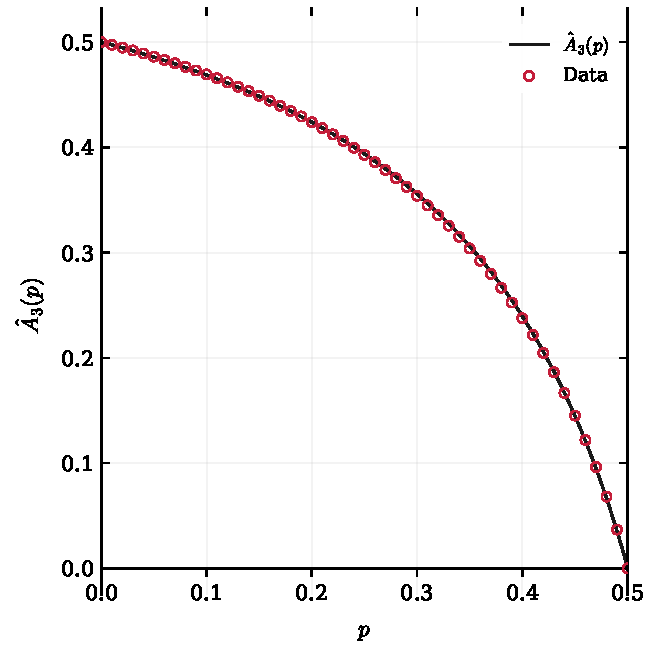
\includegraphics[width=0.56\textwidth]{figures/IMG_ch3/A3_hat_plot.pdf}
\caption{Symbolic-regression candidate \(\hat A_3(p)\) of \cref{eq:A3hat} (solid) against numerical \(A(p)\) (red circles). Visual agreement is excellent; \(\hat A_3(\tfrac12)=9.1\times10^{-4}\) rather than \(0\), and the critical gradient is \(-3.63\) rather than \(-4\). Errors of this size devastate \(1/A\) near criticality.}
\label{fig:A3hat}
\end{figure}

The recurring defect is failure to hit \((\tfrac12,0)\) with gradient \(-4\). As \(A\to0\), an absolute error that vanishes on a plot of \(A\) produces an \(O(1)\) and eventually unbounded error in the quasi-stationary mean \(1/A\).

A pragmatic splice of a fitted curve onto the asymptotic, for example
\begin{equation}
\label{eq:A4hat}
\hat A_4(p) =
\begin{cases}
-0.04011483983619545\,\ee^{\ee^{2p}} + 0.6079994336528085, & p < 0.499962,\\[2mm]
2-4p, & p \ge 0.499962,
\end{cases}
\end{equation}
works numerically, but if one is to splice it is better to splice onto something exact; \cref{sec:practical} does so. The deeper lesson is that curve-fitting cannot distinguish a function with a closed form from one without: many radically different expressions track \(A(p)\) closely on a bounded interval.

\subsection{The Koenigs connection}
\label{sec:koenigs}

A dynamical argument explains why no elementary closed form should be expected: \(A(p)\) is a value of the Koenigs linearising function of the logistic map, and that function is non-elementary throughout the parameter range of interest.

\begin{definition}[Koenigs function]
\label{def:koenigs}
Let \(f(z) = rz(1-z)\) have a fixed point at \(z=0\) with multiplier \(r = f'(0)\), and suppose \(|r|\notin\{0,1\}\). Koenigs \cite{Koenigs1884} proved that there exists a unique function \(\psi_r\), analytic near the origin, satisfying the Schr\"oder equation
\begin{equation}
\label{eq:schroder}
\psi_r\bigl(f(z)\bigr) = r\,\psi_r(z),
\qquad
\psi_r(0)=0,
\qquad
\psi_r'(0)=1 .
\end{equation}
\end{definition}

The Koenigs function is a change of coordinate that straightens the dynamics: in the \(\psi\) coordinate the nonlinear map \(f\) becomes multiplication by \(r\) (\cref{fig:koenigs}). Here \(f(z)=rz(1-z)\) is exactly \cref{eq:logistic}, with multiplier \(r=2p\in(0,1)\).

\begin{figure}[ht]
\centering
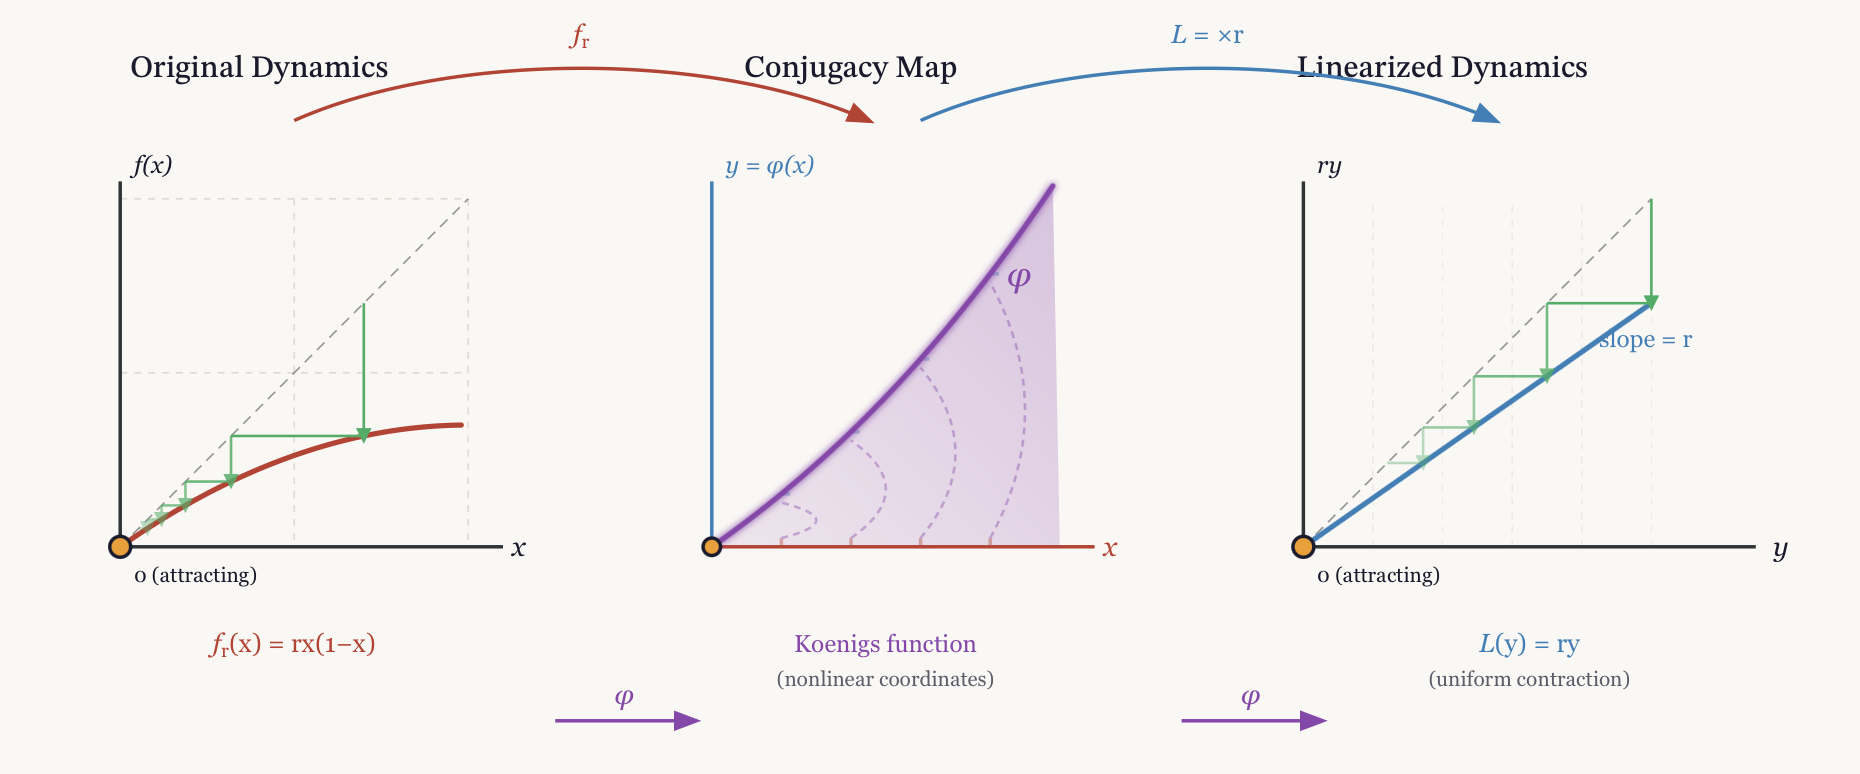
\includegraphics[width=0.72\textwidth]{figures/IMG_ch3/figure2_koenigs_linearization.png}
\caption{Koenigs linearisation of the logistic map near an attracting fixed point: \(\psi_r(f_r(x))=r\psi_r(x)\).}
\label{fig:koenigs}
\end{figure}

\begin{proposition}
\label{prop:AisKoenigs}
For \(p\in(0,\tfrac12)\) and \(r=2p\),
\begin{equation}
\label{eq:AeqKoenigs}
A(p) = 2\,\psi_r\!\lrb{\tfrac12}.
\end{equation}
\end{proposition}

\begin{proof}
Iterating \cref{eq:schroder} along the orbit \(w_n\) of \cref{eq:logistic} gives \(\psi(w_0)=\psi(w_n)/r^n\) for every \(n\). Passing to the limit and using \(\psi(z)/z\to1\) as \(z\to0\) with \(w_n\to0\) yields \(\psi(w_0)=\lim_n w_n/r^n\). Comparing with \cref{eq:Aw} and \(w_0=\tfrac12\) gives \(A(p)=2\psi_r(\tfrac12)\).
\end{proof}

\subsubsection*{When is \texorpdfstring{$\psi_r$}{psi} elementary?}

Essentially never. The logistic family is affinely conjugate to the quadratic family \(P_c(z)=z^2+c\); substituting \(x=-z/r+\tfrac12\) in \(f_r\) gives \(P_c\) with
\begin{equation}
\label{eq:cofr}
c = \frac{2r-r^2}{4}.
\end{equation}
Under this correspondence, \(r\in(0,1)\) maps to \(c\in(0,\tfrac14)\) (\cref{fig:conjugacy}). Becker and Bergweiler \cite{Becker1995} proved that for a rational map of degree at least two with fixed-point multiplier \(\lambda\), \(0<|\lambda|<1\), the associated Koenigs linearisation satisfies an algebraic differential equation only when the map is analytically conjugate to a monomial \(z\mapsto z^{\pm d}\) or a Chebyshev polynomial \(\pm T_d\). For the quadratic family the exceptional cases are \(c=0\) and \(c=-2\), corresponding to \(r=2\) and \(r=4\).

Every elementary function in the Liouville sense satisfies an algebraic differential equation. A hypertranscendental function satisfies none. Since
\begin{equation*}
\lrb{0,\tfrac14}\cap\{0,-2\} = \emptyset,
\end{equation*}
no \(r\) in the branching window is exceptional: for each fixed \(r\in(0,1)\), \(\psi_r\) is hypertranscendental and in particular not elementary.

\begin{figure}[ht]
\centering
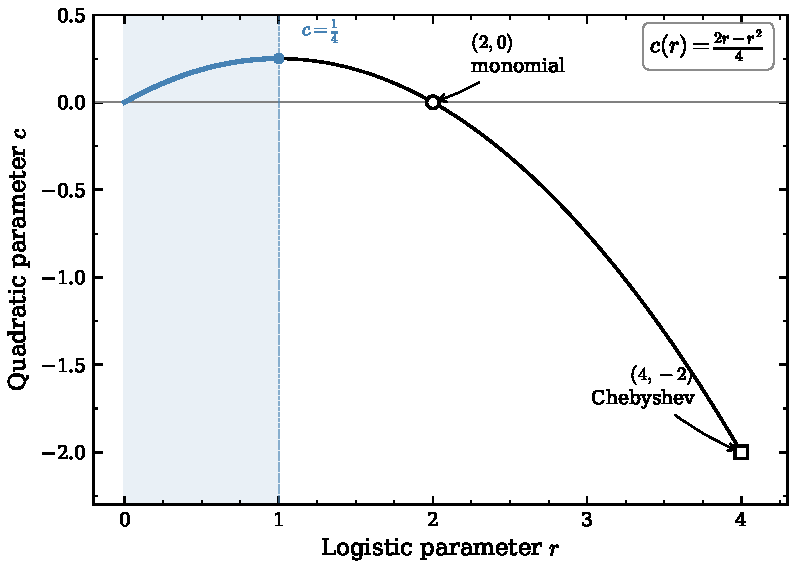
\includegraphics[width=0.66\textwidth]{figures/IMG_ch3/figure1_parameter_conjugacy.pdf}
\caption{Parameter correspondence \(c(r)=(2r-r^2)/4\) between the logistic and quadratic families. The shaded segment \(r\in(0,1)\) maps to \(c\in(0,\tfrac14)\). The integrable parameters \(r=2\) (\(c=0\)) and \(r=4\) (\(c=-2\)) lie outside it.}
\label{fig:conjugacy}
\end{figure}

\paragraph{The monomial case, \(r=2\).}
Here \(f_2(x)=2x(1-x)\). The substitution \(u=1-2x\) gives \(u\mapsto u^2\), linearised by the logarithm. Returning to \(x\) and imposing the Koenigs normalisation,
\begin{equation}
\label{eq:psi2}
\psi_2(x) = -\tfrac12\ln(1-2x).
\end{equation}

\paragraph{The Chebyshev case, \(r=4\).}
Here \(f_4(x)=4x(1-x)\) is conjugate to angle doubling via \(x=\sin^2\theta\), and
\begin{equation}
\label{eq:psi4}
\psi_4(x) = \bigl(\arcsin\sqrt{x}\,\bigr)^2 .
\end{equation}

\begin{remark}[Attracting versus repelling]
\label{rem:attractrepel}
At \(r=2\) and \(r=4\) the multiplier satisfies \(|r|>1\), so the origin is repelling. The functions \cref{eq:psi2,eq:psi4} are Poincar\'e-type linearisations rather than attracting-Koenigs maps, and neither parameter lies in \(r=2p\in[0,1)\). They illustrate solvable cases; they do not bear on \(A(p)\).
\end{remark}

\subsubsection*{What this does and does not establish}

For each fixed \(r\in(0,1)\), \(z\mapsto\psi_r(z)\) is hypertranscendental. Combined with \cref{prop:AisKoenigs}, \(A(p)\) is a value of a non-elementary function at \(z=\tfrac12\). This strongly indicates that the searches of \cref{sec:GA} were doomed.

What is \emph{not} established is that the map \(p\mapsto A(p)\) admits no elementary description: hypertranscendence of \(\psi_r\) in its argument is logically distinct from transcendence of the values \(2\psi_{2p}(\tfrac12)\). No rigorous negative result for \(p\mapsto A(p)\) is claimed. The honest summary is that no closed form is known, that the structural reason for expecting none is the one just given, and that the numerical evidence is consistent with there being none.

Under \(c=\lambda/2-\lambda^2/4\), the branching window \(r\in(0,1)\) is the real diameter of the main cardioid of the Mandelbrot set, from the centre \(c=0\) out to the parabolic cusp \(c=\tfrac14\) (criticality). \Cref{fig:mandelbrot} places the segment in context. Throughout the window the Julia set is a quasicircle bounding the basin of the attracting fixed point, and the Koenigs function is the conformal coordinate that linearises the dynamics inside that basin. A function whose natural domain has no smooth description is a poor candidate for a closed form; \(A(p)\), being one of its values, inherits the difficulty.

\begin{figure}[ht]
\centering
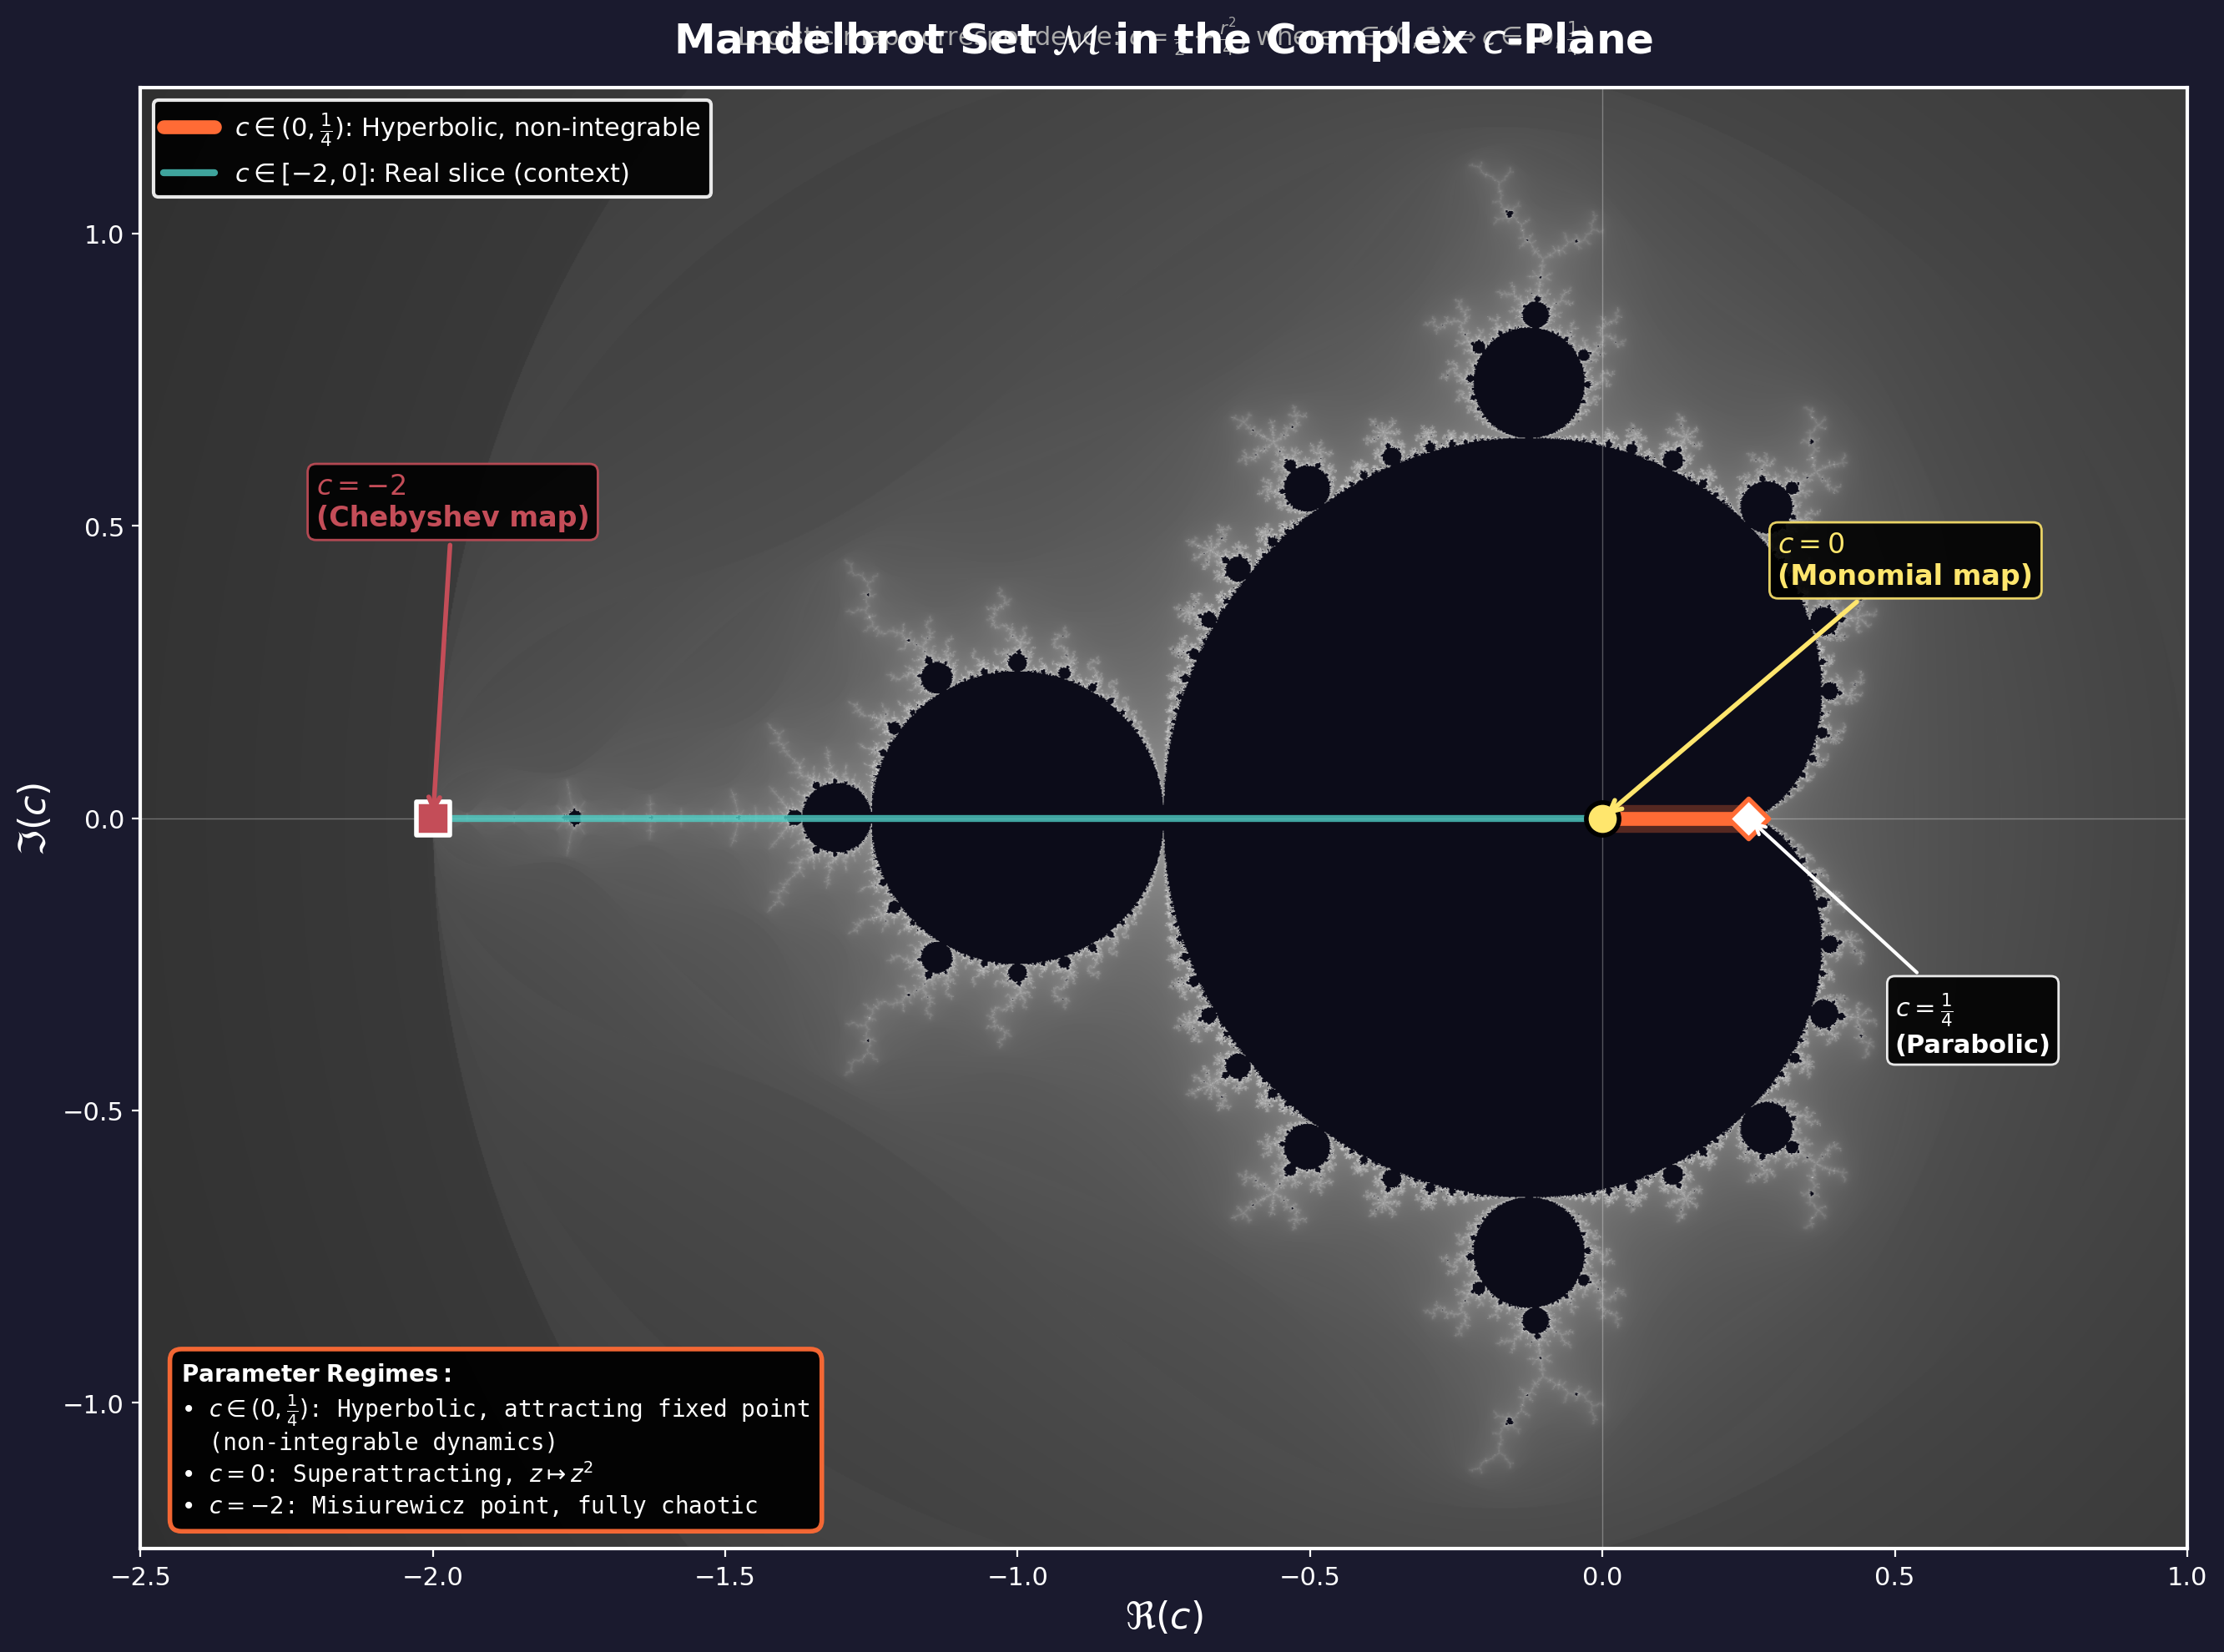
\includegraphics[width=0.92\textwidth]{figures/IMG_ch3/figure4_mandelbrot_context.png}
\caption{The Mandelbrot set with the interval \(c\in(0,\tfrac14)\) highlighted --- the image of the subcritical branching window under \(c=(2r-r^2)/4\). Integrable parameters \(c=0\) and \(c=-2\) are marked.}
\label{fig:mandelbrot}
\end{figure}

\subsection{Computing \texorpdfstring{$A(p)$}{A(p)} in practice}
\label{sec:practical}

In the absence of an exact formula one approximates, splitting the interval into regimes suggested by \cref{sec:Abounds}.

Over most of the range, the infinite product \cref{eq:prodFormula} converges quickly and partial products bound \(A(p)\) from above. Difficulty is confined to a neighbourhood of \(p=\tfrac12\): as \(A\to0\), absolute errors in \(A\) become unbounded errors in \(1/A\); and as criticality is approached, \(S_n\) recedes to zero ever more slowly. \Cref{tab:Avals} records the cost: of order \(10^2\) iterations at \(p=0.2\), \(10^3\) at \(p=0.45\), and nearly \(5\times10^5\) at \(p=0.4999\).

The remedy is to hand the near-critical region to the asymptotic \cref{eq:Aasym}:
\begin{equation}
\label{eq:Apractical}
A(p) \approx
\begin{cases}
\displaystyle \frac12\prod_{k=1}^{N}\lrb{1-\frac{S_k}{2}}, & p<c,\quad N\gg1,\\[14pt]
2-4p, & p\ge c,
\end{cases}
\end{equation}
with crossover \(c\) just below \(\tfrac12\). At \(c=0.4999\) (\(\varepsilon=2\times10^{-4}\)) the relative error of the asymptotic is of order a few parts in \(10^3\), while the product still converges in a few hundred thousand iterations. Any \(c\) in \(0.499\)--\(0.4999\) yields accuracy better than one per cent throughout. This is the recipe underlying the numerical values quoted in this chapter, including those in \cref{fig:condmean,tab:Avals}.

\FloatBarrier

\section{Absorption models and the method of characteristics}
\label{sec:moc}

Birth--death dynamics of pathogenic particles inside a host cell that can rupture leave open the question of what happens when several hosts share a medium and the first cell ruptures. Immediate transfer of the entire intracellular load into another host is a strong modelling assumption. A more realistic alternative is an \emph{absorption period}: following rupture, absorption events redistribute the released cohort among remaining hosts before intracellular birth, death, and rupture resume. Working towards such models, we begin with a pathogenic cohort infiltrating a single host cell.

Three models are treated in increasing order of difficulty. In the first two, particles are conserved or only lost, the state space is finite, and independence delivers the generating function without solving a partial differential equation. In the third, intracellular replication opens an infinite state space, the independence shortcut fails as a computational device, and the PDE must be solved by the method of characteristics. Characteristics are first tested on absorption--death, where the answer is already known, and then applied to absorption--birth--death.

\subsection{Absorption only}
\label{sec:absonly}

The simplest process has a single host that absorbs particles, with no birth or death of pathogen within the host. Let \(\xt\) and \(\yt\) denote intracellular and extracellular counts. Inter-event times are exponential, so \(\{(\xt,\yt):t\ge0\}\) is a continuous-time Markov chain.

Over an infinitesimal interval \(\Delta t\),
\begin{align*}
     \pr{\Delta\xx= 1,\;\Delta\yy = -1 \;|\; \yt = j} &= j \alpha \Delta t,  &&\text{(absorption)}\\
     \pr{\Delta\xx= 0,\;\Delta\yy = 0 \;|\; \yt = j} &= 1 -  j \alpha \Delta t,  &&\text{(no event)}
\end{align*}
with initial condition \(\xx_0=0\), \(\yy_0=N\). Writing \(\pt=\pr{\xt=i,\ \yt=j}\), the forward Kolmogorov equations are
\begin{equation}
\label{F1}
\ddt{\p} = \alpha(j+1)p_{i-1,j+1} - \alpha j\,\p .
\end{equation}
With the generating function
\begin{equation}
\label{pgfDef}
G(x,y,t) = \sum_i\sum_j \pt\, x^iy^j
=\mean{x^{\xt}y^{\yt}},
\end{equation}
multiplying \cref{F1} by \(x^iy^j\), summing, and rearranging produces the first-order PDE
\begin{equation}
\label{PDE1}
\pddt{G(x,y,t)} = \alpha\left(x - y\right) \pdd{G(x,y,t)}{y},
\qquad G(x,y,0) = y^N .
\end{equation}
Particles are neither created nor destroyed, so \(\pt=0\) whenever \(i+j\neq N\).

\subsubsection*{Exploiting independence}

Define more generally
\begin{equation*}
G_n(x,y,t) = \sum_i\sum_j \pr{\xt = i,\;\yt=j \;|\;\xx_0 = 0,\;\yy_0=n } x^i y^j .
\end{equation*}
In pure absorption the \(n\) particles move independently, so
\begin{equation}
\label{indRelPGF}
G_n(x,y,t) = \bigl(G_1(x,y,t)\bigr)^n .
\end{equation}
For a single particle, the only reachable states have \(i+j=1\), and
\begin{align*}
p_{0,1}(t) = \ee^{-\alpha t}, && p_{1,0}(t) = 1 - \ee^{-\alpha t} .
\end{align*}

\begin{figure}[H]
\centering
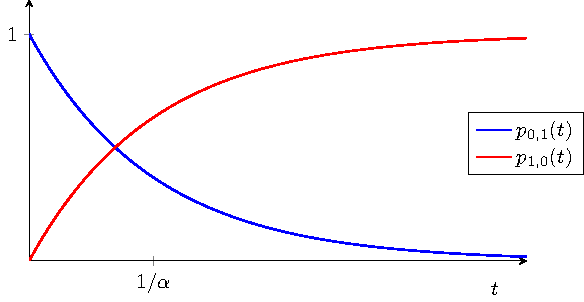
\includegraphics[width = 0.62\textwidth]{figures/IMG_ch3/abs1.pdf}
\caption{Single-particle absorption-only state probabilities: \(p_{0,1}\) decays exponentially at rate \(\alpha\); \(p_{1,0}\) rises to one.}
\label{fig:abs1}
\end{figure}

Hence
\begin{equation*}
G_1(x,y,t) = \lrb{1-\ee^{-\alpha t}}x + \ee^{-\alpha t}y ,
\end{equation*}
and
\begin{equation}
\label{eq:Gabsonly}
G_n(x,y,t) = \Bigl(\lrb{1-\ee^{-\alpha t}}x + \ee^{-\alpha t}y\Bigr)^n .
\end{equation}
This satisfies \cref{PDE1} with \(G_n(x,y,0)=y^n\). Equivalently, \(\xt\sim\mathrm{Binomial}(n,1-\ee^{-\alpha t})\).

\subsection{Absorption--death}
\label{sec:absdeath}

A particle inside the host may die. Transitions become
\begin{align*}
     \pr{\Delta\xx= 1,\;\Delta\yy = -1 \;|\; \yt = j} &= j \alpha \Delta t,  &&\text{(absorption)}\\
      \pr{\Delta\xx= -1,\;\Delta\yy = 0 \;|\; \xt = i} &= i \mu \Delta t,  &&\text{(death)}\\
     \pr{\Delta\xx= 0,\;\Delta\yy = 0 \;|\; \yt = j,\, \xt=i} &= 1 -  \lrb{ j\alpha + i\mu}\Delta t,
\end{align*}
with forward equations
\begin{equation}
\label{FK1}
\ddt{\p} = \alpha(j+1)p_{i-1,j+1} + \mu(i+1)p_{i+1,j} - (\alpha j + \mu i)\p
\end{equation}
and generating-function PDE
\begin{equation}
\label{PDE2}
\pddt{G(x,y,t)} = \mu(1-x)\pdd{G(x,y,t)}{x} + \alpha\left(x - y\right)\pdd{G(x,y,t)}{y},
\qquad G(x,y,0)=y^N.
\end{equation}
Independence still holds. For one particle,
\begin{align}
\label{eq:absdeathstates}
p_{0,1}(t) = \ee^{-\alpha t}, &&
p_{1,0}(t) = \frac{\alpha}{\mu - \alpha}\Bigl(\ee^{-\alpha t} - \ee^{-\mu t}\Bigr), &&
p_{0,0}(t) = 1 - p_{0,1}(t) - p_{1,0}(t).
\end{align}

\begin{figure}[H]
\centering
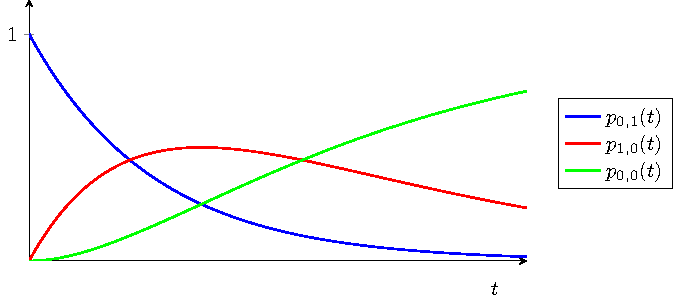
\includegraphics[width = 0.62\textwidth]{figures/IMG_ch3/abs2.pdf}
\caption{Single-particle absorption--death probabilities: outside (blue), inside (red), dead (green).}
\label{fig:abs2}
\end{figure}

The general generating function is
\begin{equation}
\label{eq:Gabsdeath}
G_n(x,y,t) = \Bigl(1-\tfrac{\mu}{\mu - \alpha}\ee^{-\alpha t} + \tfrac{\alpha}{\mu - \alpha}\ee^{-\mu t}
+ \tfrac{\alpha}{\mu - \alpha}\bigl(\ee^{-\alpha t} - \ee^{-\mu t}\bigr)x + \ee^{-\alpha t}y\Bigr)^n .
\end{equation}

\subsection{The method of characteristics, tested on absorption--death}
\label{sec:mocabsdeath}

Before treating absorption--birth--death, where independence no longer yields a finite closed form for \(G_1\), we re-derive \cref{eq:Gabsdeath} from the PDE by characteristics, as a controlled test.\footnote{I am grateful to Benjamin Sharp for advice on applying the method of characteristics to three-variate problems that unlocked this development.}

Introduce \((x,y,t)\to(s,r,\tau)\) with \(G\) regarded as a function of \(\tau\) alone along characteristics of constant \(s,r\). The initial surface is
\begin{equation}
\label{ICpar}
x(s,r,0) = s, \qquad y(s,r,0) = r, \qquad t(s,r,0) = 0 .
\end{equation}
Comparing the chain rule for \(\mathrm{d}G/\mathrm{d}\tau\) with \cref{PDE2} written as
\begin{equation*}
0 = -\pddt{G} + \mu(1-x)\pdd{G}{x} + \alpha(x-y)\pdd{G}{y}
\end{equation*}
produces the characteristic system
\begin{align}
\dda{G}{\tau} &= 0, \label{ch11}\\
\dda{t}{\tau} &= -1, \label{ch12}\\
\dda{x}{\tau} &= \mu(1-x), \label{ch13}\\
\dda{y}{\tau} &= \alpha(x-y). \label{ch14}
\end{align}

\paragraph{The equation for \(G\), \eqref{ch11}.}
\(G\) is constant along characteristics. With \(G(s,r,0)=r^N\),
\begin{equation}
\label{GrN}
G(s,r,\tau) = r^N .
\end{equation}
The problem reduces to expressing \(r\) in terms of \((x,y,t)\).

\paragraph{The equation for \(t\), \eqref{ch12}.}
\begin{equation}
\label{minustau}
t = -\tau .
\end{equation}
The characteristic parameter runs backwards in time, so the initial surface is reachable from any \((x,y,t)\).

\paragraph{The equation for \(x\), \eqref{ch13}.}
\begin{equation}
\label{sandxwithtau}
1-x = (1-s)\ee^{-\mu\tau} .
\end{equation}

\paragraph{The equation for \(y\), \eqref{ch14}.}
Solving with integrating factor \(\ee^{\alpha\tau}\) and imposing \cref{ICpar} yields
\begin{equation}
\label{ywithr1}
y = 1 - \frac{\alpha}{\alpha-\mu}(1-s)\ee^{-\mu\tau} + \lrb{r + \frac{\alpha}{\alpha-\mu}(1-s) - 1}\ee^{-\alpha\tau}.
\end{equation}

\paragraph{Recovering the solution.}
Solving \cref{ywithr1} for \(r\), substituting \(s\) from \cref{sandxwithtau} and \(\tau=-t\), and applying \cref{GrN} reproduces \cref{eq:Gabsdeath} exactly. The two routes agree; the machinery is ready for the case where only one is available.

\subsection{Absorption--birth--death}
\label{sec:absbirthdeath}

With intracellular replication, infinitely many states are reachable from a single particle, so \(G_1\) is an infinite series and factorisation no longer simplifies the computation. The PDE must be solved directly.

Transitions:
\begin{align*}
     \pr{\Delta\xx= 1,\;\Delta\yy = -1 \;|\; \yt = j} &= j \alpha \Delta t,  &&\text{(absorption)}\\
     \pr{\Delta\xx= 1,\;\Delta\yy = 0 \;|\; \xt = i} &= i \beta \Delta t,  &&\text{(birth)}\\
      \pr{\Delta\xx= -1,\;\Delta\yy = 0 \;|\; \xt = i} &= i \mu \Delta t,  &&\text{(death)}\\
     \pr{\Delta\xx= 0,\;\Delta\yy = 0 \;|\; \yt = j,\, \xt=i} &= 1 -  \lrb{ j\alpha + i\mu + i\beta}\Delta t,
\end{align*}
with forward equation
\begin{equation}
\label{FK3}
\pddt{\p} = \alpha(j+1)p_{i-1,j+1} + \mu(i+1)p_{i+1,j} + \beta(i-1)p_{i-1,j} - (\alpha j + \mu i + \beta i)\p
\end{equation}
and generating-function PDE
\begin{equation}
\label{PDE3}
\pddt{G} = \lrb{\mu - (\mu+\beta)x + \beta x^2}\pdd{G}{x} + \alpha(x-y)\pdd{G}{y},
\qquad G(x,y,0) = y^N .
\end{equation}
The characteristic system is
\begin{align}
\dda{G}{\tau} &= 0, \label{ch21}\\
\dda{t}{\tau} &= -1, \label{ch22}\\
\dda{x}{\tau} &= \mu-(\mu+\beta)x + \beta x^2, \label{ch23}\\
\dda{y}{\tau} &= \alpha(x-y), \label{ch24}
\end{align}
with initial surface \cref{ICpar}.

\paragraph{The equations for \(G\) and \(t\), \eqref{ch21}--\eqref{ch22}.}
\begin{equation}
\label{gngngn}
G(s,r,\tau) = r^N,
\qquad t = -\tau .
\end{equation}

\paragraph{The equation for \(x\), \eqref{ch23}.}
The right-hand side is Riccati and factorises as
\begin{equation}
\label{eq:xpm}
\mu - (\mu+\beta)x + \beta x^2 = \beta(x-x_+)(x-x_-),
\qquad
x_+ = 1,\quad x_- = \frac{\mu}{\beta}.
\end{equation}
Write \(b_1=\beta-\mu\) for the net intracellular growth rate. Separating variables and applying \cref{ICpar} gives
\begin{equation}
\label{eq:xratio}
\frac{x-x_+}{x-x_-} = \lrb{\frac{s-x_+}{s-x_-}}\ee^{b_1\tau},
\end{equation}
or
\begin{equation}
\label{xabd}
x(\tau) = \frac{x_+(s-x_-) - x_-(s-x_+)\ee^{b_1\tau}}{(s-x_-) - (s-x_+)\ee^{b_1\tau}} .
\end{equation}

\paragraph{The equation for \(y\), \eqref{ch24}.}
With integrating factor,
\begin{equation}
\label{eq:yint}
\dda{}{\tau}\lrb{\ee^{\alpha\tau}y} = \alpha\,\ee^{\alpha\tau}x(\tau).
\end{equation}
Expanding \(x(\tau)\) as a geometric series in
\begin{equation*}
\zeta(\tau) = \lrb{\frac{s-x_+}{s-x_-}}\ee^{b_1\tau}
\end{equation*}
yields term-by-term integrals and defines
\begin{equation}
\label{eq:Psidef}
\Psi(\zeta) \;=\; x_+ + \frac{\alpha}{\beta}\sum_{n=1}^{\infty}\frac{\zeta^{\,n}}{n+\delta},
\qquad \delta = \frac{\alpha}{b_1} = \frac{\alpha}{\beta-\mu}.
\end{equation}
Imposing the initial condition for \(y\) and restoring \((x,y,t)\) produces the closed form.

\begin{proposition}[Generating function for absorption--birth--death]
\label{prop:Gabd}
With \(x_+=1\), \(x_-=\mu/\beta\), \(b_1 = \beta-\mu\), \(\delta = \alpha/b_1\),
\(W = (x-x_+)/(x-x_-)\) and \(\Psi\) as in \cref{eq:Psidef},
\begin{equation}
\label{eq:Gabd}
\boxed{\;
G(x,y,t) = \Bigl\{\ee^{-\alpha t}\bigl[y - \Psi(W)\bigr] + \Psi\bigl(W\ee^{b_1 t}\bigr)\Bigr\}^{N}. \;}
\end{equation}
\end{proposition}

Three checks confirm the result. At \(t=0\) the \(\Psi\) terms cancel and \(G=y^N\). At \(x=y=1\), \(W=0\) and \(\Psi(0)=1\), so \(G=1\). Setting \(x=1\) alone gives
\begin{equation*}
G(1,y,t) = \bigl(\ee^{-\alpha t}y + 1 - \ee^{-\alpha t}\bigr)^N,
\end{equation*}
so \(\yt\sim\mathrm{Binomial}(N,\ee^{-\alpha t})\), as required by independent extracellular absorption. Beyond these, \cref{eq:Gabd} has been verified numerically against direct integration of \cref{FK3}, agreeing to around \(10^{-13}\) across sub- and supercritical intracellular regimes for \(N=1,2,3\).

\subsubsection*{Hypergeometric form}

The series in \cref{eq:Psidef} is a Gauss hypergeometric function. With the Pochhammer symbol \((q)_n\),
\begin{equation}
\label{eq:2F1def}
{}_2F_1(a,b;c;z) = \sum^\infty_{n=0}\frac{(a)_n(b)_n}{(c)_n}\frac{z^n}{n!},
\end{equation}
the case \(a=1\), \(b=\delta\), \(c=\delta+1\) collapses to
\begin{equation}
\label{eq:2F1simple}
{}_2F_1\lrb{1,\delta;\delta+1;z} = \sum_{n=0}^{\infty}\frac{\delta}{\delta+n}z^n ,
\end{equation}
and
\begin{equation}
\label{eq:Psihyp}
\Psi(\zeta) = x_+ + (x_+-x_-)\Bigl[{}_2F_1\lrb{1,\delta;\delta+1;\zeta} - 1\Bigr].
\end{equation}
An alternative derivation of the same object via the integral \(\int\ee^{h\tau}/(p+q\ee^{k\tau})\,\mathrm{d}\tau\) is given in \cref{app:hyp}. Coefficient extraction from multilinear generating functions is recorded in \cref{app:extract}.

\begin{remark}[Domain of validity]
\label{rem:domain}
The series \cref{eq:Psidef} converges for \(|\zeta|<1\). In the subcritical intracellular regime \(\mu>\beta\), \(b_1<0\) and \(x_->1\), so for \(x\in[0,1]\) the arguments in \cref{eq:Gabd} lie in the unit disk. When \(\beta>\mu\) one uses the analytic continuation of \({}_2F_1\), for example the Euler integral representation.
\end{remark}

\begin{remark}[Resonance]
\label{rem:resonance}
Denominators in \cref{eq:Psidef} vanish when \(\alpha=n(\mu-\beta)\) for some integer \(n\ge1\). This is a removable resonance of the linearised \(y\)-equation; the generating function itself remains analytic in the parameters, and the corresponding term acquires a secular factor \(\tau\) in place of a pure exponential.
\end{remark}

\FloatBarrier

\appendix
\section*{Appendices}
\addcontentsline{toc}{section}{Appendices}
\renewcommand{\thesubsection}{\Alph{subsection}}
\setcounter{subsection}{0}

\subsection{An integral identity for the hypergeometric function}
\label{app:hyp}

An alternative route to \cref{eq:Psidef} integrates the characteristic \(x(\tau)\) as a quotient, splitting the numerator into pieces of the form
\begin{equation}
\label{eq:Iform}
I(\tau) = \int\frac{\ee^{h\tau}}{p+q\,\ee^{k\tau}}\,\dd\tau ,
\end{equation}
with \(h,k,p,q\) constant. The bookkeeping is longer than the geometric-series expansion of \cref{sec:absbirthdeath}, but the identity is useful in its own right.

\begin{proposition}
\label{prop:hypIden}
For \(h/k>0\) and \(-\tfrac{q}{p}\ee^{k\tau}\notin[1,\infty)\),
\begin{equation}
\label{hypIden}
\int\frac{\ee^{h\tau}}{p+q\ee^{k\tau}}\,\dd\tau
= \frac{\ee^{h\tau}}{ph}\,{}_2F_1\lrb{1,\frac{h}{k};\frac{h}{k}+1;\,-\frac{q}{p}\ee^{k\tau}} + \text{const}.
\end{equation}
\end{proposition}

\begin{proof}
Use the Euler integral representation
\begin{equation}
\label{idenHyp}
{}_2F_1(a,b;c;z) = \frac{\Gamma(c)}{\Gamma(b)\Gamma(c-b)}\int^1_0 u^{b-1}(1-u)^{c-b-1}(1-zu)^{-a}\,\dd u .
\end{equation}
Substitute \(v=\ee^{k\tau}\) in \cref{eq:Iform}, so \(\mathrm{d}\tau=k^{-1}v^{-1}\mathrm{d}v\):
\begin{equation*}
I = \frac{1}{pk}\int\frac{v^{h/k-1}}{1+(q/p)v}\,\dd v .
\end{equation*}
Writing the antiderivative as a definite integral from \(0\) to \(v\) (convergent at the lower limit because \(h/k>0\)) and rescaling \(w=vu\) produces
\begin{equation*}
I = \frac{v^{h/k}}{pk}\int_0^1\frac{u^{h/k-1}}{1+(q/p)vu}\,\dd u .
\end{equation*}
The integrand matches \cref{idenHyp} with \(a=1\), \(b=h/k\), \(c=h/k+1\), \(z=-(q/p)v\). Using \(\Gamma(z+1)=z\Gamma(z)\) and restoring \(v=\ee^{k\tau}\) yields \cref{hypIden}.
\end{proof}

\begin{remark}
Applied to the two pieces of \cref{xabd} --- the first with \(h=\alpha\), the second with \(h=\alpha+b_1\), both with \(k=b_1\), \(p=(s-x_-)\), \(q=-(s-x_+)\) --- \cref{prop:hypIden} reproduces \cref{eq:Psihyp} after prefactors are carried correctly. Checking \(G(1,1,t)=1\) catches dropped factors invisible at \(t=0\).
\end{remark}

\subsection{Extracting state probabilities from a generating function}
\label{app:extract}

A generating function defined by a closed formula rather than an explicit series, for example
\begin{equation}
\label{examplePgf}
G(t;x,y) = \Bigl(\bigl(1-\ee^{-\alpha t}\bigr)x + \ee^{-\alpha t}y\Bigr)^n ,
\end{equation}
converts back to
\begin{equation}
\label{series1}
G(t;x,y) = \sum^{\infty}_{i=0}\sum^{\infty}_{j=0} p_{i,j}(t)\,x^iy^j
\end{equation}
by repeated partial differentiation, whenever the derivatives exist:
\begin{equation}
\label{stateProb}
p_{i,j}(t) = \frac{1}{i!\,j!}\,\partial_x^i\partial_y^{\,j}G\Big|_{(0,0)} .
\end{equation}

\subsubsection*{The multilinear case}

Both \cref{eq:Gabsonly} and \cref{eq:Gabsdeath} have the form
\begin{equation}
\label{eq:multilinear}
G(t;x,y) = \bigl(c(t) + f(t)\,x + g(t)\,y\bigr)^n .
\end{equation}
Differentiation yields
\begin{equation}
\label{eq:derivs}
\partial_x^{a}\partial_y^{\,b}G = \frac{n!}{(n-a-b)!}\,f^{a}g^{b}\bigl(c+fx+gy\bigr)^{n-a-b}
\qquad (a+b\le n),
\end{equation}
and evaluating at the origin gives the trinomial probabilities
\begin{equation}
\label{stateProbSpec}
p_{i,j}(t) = \frac{n!}{i!\,j!\,(n-i-j)!}\;f(t)^{i}\,g(t)^{j}\,c(t)^{\,n-i-j},
\qquad i+j\le n.
\end{equation}
This is the joint law of \(n\) independent particles, each ending in one of three states with probabilities \(c\), \(f\), and \(g\).

\subsubsection*{Applied to the absorption models}

For absorption only, \(c=0\), \(f=1-\ee^{-\alpha t}\), \(g=\ee^{-\alpha t}\), and \cref{stateProbSpec} recovers the binomial law of \cref{sec:absonly}. For absorption--death the three functions \(c,f,g\) are exactly \(p_{0,0}\), \(p_{1,0}\), and \(p_{0,1}\) of \cref{eq:absdeathstates}, and the joint law is trinomial. The absorption--birth--death generating function of \cref{prop:Gabd} is not multilinear; there \cref{stateProb} must be applied to \cref{eq:Gabd} directly, or coefficients extracted numerically by Cauchy integrals on circles \(|x|=|y|=\rho<1\).


\FloatBarrier
\begingroup
\footnotesize
\bibliographystyle{unsrt}
\bibliography{references}
\endgroup

\end{document}
